% Modified 31 Oct 2005:  Conditioning fallacy alluded to.
% This chapter has been modified on 6-4-05.
% There are two \choice
\pagestyle{headings}
\chapter{Random Variables} \label{chp 4}

\section{Discrete Random Variables}\label{RVIntroSec}

\begin{definition}\index{Random Variable}\label{RandomVariableDef} A \newterm{random variable} is a function from a sample space $\Omega$ to $\mathbb{R}$. If the range of this function is countable, the random variable is called discrete. In this section, we'll deal only with discrete random variables.
\end{definition}

Since a sample space is used to represent the possible outcomes of an experiment, a random variable associates a real number with each possible outcome. In other words, a random variable is a variable whose value is determined by the outcome of an experiment involving some element of chance.

Random variables are typically denoted using capital letters at the end of the alphabet, such as $X$, $Y$, or $Z$, and the probability the random variable $X$ takes the real number value $x$ is denoted $P(X = x)$. 
%Notice that $x$ is the usual kind of real number variable you're used to dealing with in algebra and calculus, while $X$ is a random variable with an associated sample space $\Omega$ and a potentially very limited range of possible values.

\begin{example} Let $X$ denote the outcome of single roll of a fair die. Then $X$ is a random variable defined on the sample space $\Omega = \{1,2,3,4,5,6\}$.

Not surprisingly, $P(X = 1) = \frac{1}{6}$, $P(X = 2) = \frac{1}{6}$, and so on. In general, $P(X = x) = \frac{1}{6}$ for all $x \in \{1,2,3,4,5,6\}$ since the die is fair. We could also ask for $P(X > 4)$, and again you should not be surprised that $P(X > 4) = P(X=5) + P(X=6) = \frac{2}{6}$.
\end{example}

\begin{remark} It may take some time to get used to this new notation. If $X$ is a random variable, an equation like $X = 2$ or an inequality like $X > 2$ is an event, that may or may not occur depending on the value $X$ takes, so the expression $P(X = 2)$ denotes the probability of an event. \end{remark}

\begin{example} Let $Y$ denote the number of heads in three flips of a fair coin. Then $Y$ is a random variable defined on the sample space $\Omega = \{HHH, HHT, HTH, HTT, THH, THT, TTH, TTT\}$.

The range of $Y$ is $\{0,1,2,3\}$. We can calculate the probability $Y$ takes any of these values with the techniques of the previous chapter, and summarize the results in. a table.
\begin{center}
\begin{minipage}{0.4\textwidth}
$$\begin{aligned}P(Y = 0) &= P(\{TTT\}) = \textstyle\frac{1}{8} \\
P(Y = 1) &= P(\{HTT, THT, TTH\}) = \textstyle\frac{3}{8} \\
P(Y = 2) &= P(\{HHT, HTH, THH\}) = \textstyle\frac{3}{8} \\
P(Y = 3) &= P(\{HHH\}) = \textstyle\frac{1}{8}\end{aligned}$$
\end{minipage}\begin{minipage}{0.4\textwidth}
\renewcommand*{\arraystretch}{1.35}
\begin{center}
\begin{tabular}{c|c}
$y$ & $P(Y = y)$ \\
\hline
$0$ & $\frac{1}{8}$ \\
$1$ & $\frac{3}{8}$ \\
$2$ & $\frac{3}{8}$ \\
$3$ & $\frac{1}{8}$ \\
\end{tabular}
\end{center}
\renewcommand*{\arraystretch}{1}
\end{minipage}
\end{center}
\end{example}
\begin{keypoint}
When we actually perform the experiment and flip the coin three times, the random variable will take a real number value, known as a \newterm{realization}\index{Realization}. In the table above, the leftmost column is labelled with every possible realization of $Y$. Upper case letters will denote random variables, and the corresponding lower case letters will be used for realizations.
\end{keypoint}

%\begin{example} Let $X$ denote the number of hearts in three draws, with replacement, from a shuffled deck. What is $P(X > 1)$?

%We need the probability more than one heart appears in three draws, performed with replacement. Using the law of total probability / a tree diagram, we can calculate
%\eqnsgap{P(X > 1) = \frac{1}{64}+ \frac{3}{64}+ \frac{3}{64}+ \frac{3}{64} = \frac{10}{64}\approx 0.156.}
%\end{example}

%\begin{remark} Note that random variables must take real number values. If we let $X$ denote the number of heads in a single flip of a coin, then $X$ is a random variable, but if we let $X$ denote the outcome (Heads or Tails) of a single flip of a coin, then $X$ is not a random variable.
%\end{remark}

%\index{Distribution}\index{Random Variable! distribution of}The association between events that are defined in terms of a random variable $X$ and their probabilities is known as the probability distribution of $X$, which is often shortened to simply `the distribution of $X$'. There are many ways to present the distribution of a discrete random variable. One way is to simply list the possible values of $X$ and their probabilities in a table.


\subsection*{Probability Mass Functions}

%The table in the example above describes the \newterm{distribution}\index{Distribution} of the random variable $Y$, since it associates every possible value of $Y$ with a probability.

Given a random variable $X$, the function $f_X: \mathbb{R} \to \mathbb{R}$ that assigns to each possible realization of $X$ the probability it occurs (the function which is described by the table in our example above) is called the probability mass function of $X$. If $x$ is any value outside the range of $X$, then we omit this value from the table.

\begin{definition}\index{Probability Mass Function}
The \newterm{probability mass function} (abbreviated pmf) $f_X$ for the random variable $X$ is defined by $f_X(x) = P(X = x)$. We often represent this function with a table, and visualize it with a figure known as a lollipop plot.
\end{definition}

\begin{example}\label{diepairex}
Let $X$ denote the sum of the two numbers showing when a pair of fair six-sided dice is rolled. Graph the probability mass function $f_X$ with a lollipop plot.

Each die is equally likely to show any value in the set $A = \{1,2,3,4,5,6\}$, so for a pair of dice, all outcomes in $\Omega = A \times A$ occur with probability $\frac{1}{36}$. 
{\small
\begin{center}
\begin{tabular}{c|cccccc}
$_{D_1} \setminus ^{D_2}$ & 1 & 2 & 3 & 4 & 5 & 6 \\
\hline
1 & 2 & 3 & 4 & 5 & 6 & 7 \\
2 & 3 & 4 & 5 & 6 & 7 & 8 \\
3 & 4 & 5 & 6 & 7 & 8 & 9 \\
4 & 5 & 6 & 7 & 8 & 9 & $\!$10 \\
5 & 6 & 7 & 8 & 9 & $\!$10 & $\!$11 \\
6 & 7 & 8 & 9 & $\!$10 & $\!$11 & $\!$12 \\
\end{tabular}
\end{center}
}
Thus, $P(Y = 2) = \frac{1}{36}$, $P(Y = 3) = \frac{2}{36}$, $P(Y = 4) = \frac{3}{36}$, and so on. Drawing one lollipop at each realization of $X$ whose height is its probability, we obtain the lollipop plot shown below.
\begin{center}
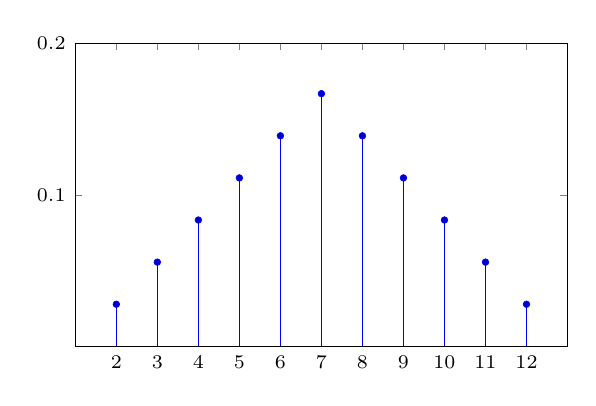
\begin{tikzpicture}[scale = 0.6]
\begin{axis} [ymin = 0, ymax = 0.2,
	tick label style={font=\scriptsize, scale = 1/0.6},
    xtick={2,3,...,12},
    ytick = {0.1,0.2},
    width=12cm, height=8cm
    ]
\addplot+[ycomb] plot coordinates {(2,1/36) (3,2/36) (4,3/36) (5,4/36) (6,5/36) (7,6/36) (8,5/36) (9,4/36)(10,3/36) (11,2/36) (12,1/36)}; 
\end{axis} 
\end{tikzpicture}
\end{center}
\end{example} 

\begin{proposition}\label{pmfproperties} Suppose that $X$ is a discrete random variable with range $A = \{x_1, x_2, x_3, \, \dots\}$. Then the probability mass function $f_X$ satisfies the following properties.
\begin{enumerate}
\item $f_X(x) \geq 0$ for all $x \in \mathbb{R}$.
\item $f_X(x) = 0$ for all $x \not\in A$.
\item $\sum_{x \in A} f_X(x) = 1$.
\end{enumerate}
\end{proposition}

\begin{remark}These properties completely characterize the class of probability mass functions for discrete random variables. In other words, if $f$ is a function with these three properties, then it is the pmf of a discrete random variable.\end{remark}

\begin{example}
Find the value of $k$ so that the function $h$ below is a pmf.
\renewcommand*{\arraystretch}{1.35}
\eqns{h(x) = \left\{
\begin{array}{cl}
      \left(\frac{1}{3k}\right)^x & \text{ if \ } x = 1, 2, 3, \dots \\
      0 & \text{otherwise} \\ \end{array} 
\right.}
\renewcommand*{\arraystretch}{1}

As long as $k$ is positive, $h$ will satisfy properties $(i)$ and $(ii)$ above. The last property allows us to determine $k$ uniquely.
$$\sum_{x \in A} h(x) =  \sum_{x = 1}^{\infty} \left(\frac{1}{3k}\right)^x = \frac{1}{3k} +  \left(\frac{1}{3k}\right)^2 +  \left(\frac{1}{3k}\right)^3 + \cdots = \frac{\frac{1}{3k}}{1-\frac{1}{3k}} = \frac{1}{3k - 1}$$

The geometric series sum formulas was used to evaluate the infinite sum. Setting the last expression equal to 1 gives $3k - 1 = 1$, and hence $k = \frac{2}{3}$. Using this value of $k$ gives the function $h$ below, which we can graph using a lollipop plot. Only the first few values can be shown, since the graph continues off to the right indefinitely.
\renewcommand*{\arraystretch}{1.35}
$$\begin{aligned}h(x) = \left\{
\begin{array}{cl}
      \left(\frac{1}{2}\right)^x & \text{ if \ } x = 1, 2, 3, \dots \\
      0 & \text{otherwise} \\ \end{array} 
\right.\end{aligned}$$

\renewcommand*{\arraystretch}{1}
\begin{center}
\begin{tikzpicture}[scale = 0.6]
\begin{axis}[ymin = 0, ymax = 0.3,
	tick label style={font=\scriptsize, scale = 1/0.6},
    xtick={2,3,...,8},
    ytick = {0.1,0.2},
    width=12cm, height=8cm]
\addplot+[ycomb] plot coordinates {(1,1/2) (2,1/4) (3,1/8) (4,1/16) (5,1/32) (6,1/64) (7,1/128) (8,1/256)}; 
\end{axis} 
\end{tikzpicture}
\end{center}
\end{example}

%\subsection*{Functions of a Discrete Random Variable}\label{FunctionsOfAnRVSec}
%\par
%If $X$ is a discrete random variable, and $g: \mathbb{R} \to \mathbb{R}$ is any function, then $Y = g(X)$ is also a discrete random variable. Its value is completely determined by the value of $X$, and given the pmf of $X$, we can determine the pmf of $Y$ by simply running all values in the range of $X$ through the function $g$. 

%\begin{example}\label{FunctionRVEx}
%Let $X$ be the random variable whose pmf is graphed below, and let $Y = 1 + X^2$ (so the function $g$ in this example is $g(x) =1+x^2$). Find the pmf of $Y$.
%\begin{center}
%\begin{tikzpicture}[scale = 0.6]
%\begin{axis}[ymin = 0, ymax = 0.4,
%xmin = -2, xmax = 4, tick label style={font=\scriptsize, scale = 1/0.6}, xtick={-2,-1,0,...,4}, ytick = {0.1,0.2,0.3,0.4}, width=12cm, height=8cm]
%\addplot+[ycomb] plot coordinates {(-1,2/10) (0,1/10) (1,2/10) (2,2/10) (3,3/10)}; 
%\end{axis} 
%\end{tikzpicture}
%\end{center}

%We calculate the realization of $Y$ that corresponds to each realization of $X$ by running them through the function $g(x) = 1+x^2$.
%\renewcommand*{\arraystretch}{1.35}
%\begin{center}
%\begin{tabular}{cc|c}
%$x$ & $y$ & $f_X(x)$ \\
%\hline
%$-1$ & $2$ & $0.2$ \\
%$0$ & $1$ & $0.1$ \\
%$1$ & $2$ & $0.2$ \\
%$2$ & $5$ & $0.2$ \\
%$3$ & $10$ & $0.3$
%\end{tabular}
%\end{center}
%\renewcommand*{\arraystretch}{1}
%Now we have a list of every possible realization of $Y$ and the probability of each. Note that there are two realizations of $X$ which result in $Y = 2$, so $f_{Y}(2) = f_X(-1) + f_X(1)$.
%\renewcommand*{\arraystretch}{1.35}
%\begin{center}
%\begin{minipage}{0.4\textwidth}
%\centering
%\begin{tabular}{c|c}
%$y$ & $f_Y(y)$ \\
%\hline
%$1$ & $0.1$ \\
%$2$ & $0.4$ \\
%$5$ & $0.2$ \\
%$10$ & $0.3$
%\end{tabular}
%\end{minipage}\begin{minipage}{0.6\textwidth}
%\centering
%\begin{tikzpicture}[scale = 0.6]
%\begin{axis}[ymin = 0, ymax = 0.5,
%xmin = 0, xmax = 11, tick label style={font=\scriptsize, scale = 1/0.6},xtick={0,1,...,11},ytick = {0.1,0.2,0.3,0.4,0.5},width=12cm, height=8cm]
%\addplot+[ycomb] plot coordinates {(1,1/10) (2,4/10) (5,2/10) (10,3/10)}; 
%\end{axis}
%\end{tikzpicture}
%\end{minipage}
%\end{center}
%\renewcommand*{\arraystretch}{1}
%\end{example}

\subsection*{Cumulative Distribution Functions}\label{DiscreteExpectationSec}

\begin{definition}\index{Cumulative Distribution Function}\index{Distribution Function}
The \newterm{cumulative distribution function} (abbreviated cdf) $F_X$ for the random variable $X$ is defined by $F_X(x) = P(X \leq x)$.
\end{definition}

Notice that we use capital letters for cdfs and lower case letters for pmfs. This is conventional and we'll always do it (for a good reason, which we'll see later). It's also worth mentioning that the word `cumulative' is frequently dropped, and the cdf is simply called the distribution function.

\begin{example} Suppose we roll a pair of dice, and let $X$ be the minimum of the two values that appear on the dice. Find the pmf $f_X$ and the cdf $F_X$.

The random variable $X$ takes integer values between 1 and 6 inclusive, and referring back to the table in Example \ref{diepairex}, we can find the probability of each realization. We have $P(X = 1) = \frac{11}{36}$ (outcomes in the first row or column), $P(X = 2) = \frac{9}{36}$ (outcomes in the second row to the right of the 3, or in the second column below the 3), $P(X = 3) = \frac{7}{36}$ (outcomes in the third row to the right of the 5, or in the third column below the 5), and so on.

The graph of the pmf $f_X$ is shown on the left, and the cdf $F_X$ is shown on the right.
\begin{center}
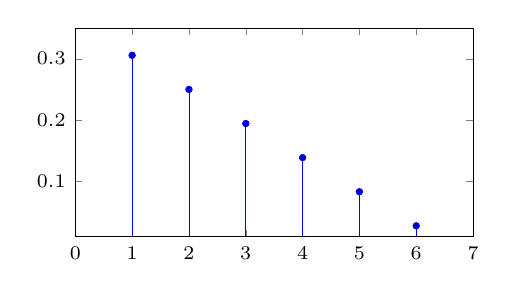
\begin{tikzpicture}[scale = 0.6]
\begin{axis} [ymin = 0.01, ymax = 0.35, xmin=0, xmax = 7,
	tick label style={font=\scriptsize, scale = 1/0.6},
    xtick={0,1,...,7},
    ytick = {0.1,0.2,0.3},
    width=10cm, height=6cm]
\addplot+[ycomb] plot coordinates {(1,11/36) (2,9/36) (3,7/36) (4,5/36) (5,3/36) (6,1/36)}; 
\end{axis} 
\end{tikzpicture}\ \ \ \ \ \  \begin{tikzpicture}[scale = 0.6]
\begin{axis}[
	tick label style={font=\scriptsize, scale = 1/0.6},
    xtick={0,1,...,7},
    ytick = {0.5,1},
    width=10cm, height=6cm,
    ymin=0,ymax=1,
    xmin=0, xmax=7,
    clip=false,
    jump mark left,
    every axis plot/.style={very thick},
    cdf,
    table/create on use/cumulative distribution/.style={
        create col/expr={\pgfmathaccuma + \thisrow{f(x)}}   
    }
]
\addplot [cdf init, blue] table [y=cumulative distribution]{
x f(x)
0 0
1 11/36
2 9/36
3 7/36
4 5/36
5 3/36
6 1/36
7 0
};
\end{axis}
\end{tikzpicture}
\end{center}

Notice that $F_X(2.5) = P(X \leq 2.5) = P(X = 1) + P(X = 2) = \frac{11}{36} + \frac{9}{36} \approx 0.56$. The cumulative distribution function adds up the probabilities that $X$ takes any value smaller than or equal to its input. 
\end{example}

Consider two real numbers $a$ and $b$ with $a \leq b$. Given any random variable $X$,  $F_X(a) \leq F_X(b)$, because if $X$ is smaller than $a$ then it must also be smaller than $b$, in other words, the event $X \leq a$ is a subset of the event $X \leq b$, and hence it cannot be more likely. This means that a cdf is always non-decreasing. This and other key properties that all cdfs share are listed in the proposition below.

\begin{proposition}\label{cdfproperties}
For any random variable $X$, the distribution function $F_X$ satisfies the following properties.
\vspace{-0.5em}
\begin{enumerate}
\item $F_X(x) \geq 0$ for all $x \in \mathbb{R}$.
\item $F_X$ is non-decreasing.
\item $\displaystyle\lim_{x \to -\infty} F_X(x) = 0$ and $\displaystyle\lim_{x \to \infty} F_X(x) = 1$.
\item $F_X(x)$ is right-continuous, meaning $\displaystyle\lim_{x \to a^{+}} F_X(x) = F_X(a)$.
\end{enumerate}
\end{proposition}

\begin{remark}These properties completely characterize the class of distribution functions, that is, any function satisfying all four properties is the cdf of some random variable.
\end{remark}

When dealing with cdfs, $F_X(a+)$ is used as an abbreviation of $\lim_{x \to a^{+}}F_X(x)$, and similarly, $F_X(a-)$ is used to abbreviate $\lim_{x \to a^{-}}F_X(x)$. Using this notation we can express the probabilities of many events succinctly in terms of the cdf.

\begin{center}
\begin{tabular}{c|c}
Event & Probability \\
\hline
$X \leq a$ & $F_X(a)$ \\
$X < a$ & $F_X(a-)$ \\
$X = a$ & $F_X(a) - F_X(a-)$ \\
$X \geq a$ & $1 - F_X(a-)$ \\
$X > a$ & $1 - F_X(a)$ \\
$a < X < b$ & $F_X(b-) - F_X(a)$ \\
$a \leq X \leq b$  & $F_X(b) - F_X(a-)$ \\
\end{tabular}
\end{center}

Of particular interest is that fact that $P(X=a) = F_X(a) - F_X(a-)$. This is a formal statement of the observation that the possible values of a discrete random variable $X$ are the values where $F_X$ has a discontinuity, and the distance the graph jumps at $a$ is $P(X = a)$.

\begin{example}
Consider the function whose graph is given below. Check that this function is a cdf for some random variable. If we call the random variable with this cdf $Z$, find $P(1 < Z < 2)$, $P(Z = 4)$, and $P(Z > 1)$.

\begin{center}
\begin{tikzpicture}[scale = 0.6]
\begin{axis}[
	tick label style={font=\scriptsize, scale = 1/0.6},
    xtick={-2,-1,...,6},
    ytick = {1/6,2/6,3/6,4/6,5/6,1},
    yticklabels = {$\frac{1}{6}$,$\frac{2}{6}$,$\frac{3}{6}$,$\frac{4}{6}$,$\frac{5}{6}$,$1$},
    width=12cm, height=8cm,
    ymin=0,ymax=1,
    xmin=0, xmax=7,
    clip=false,
    jump mark left,
    ymin=0,ymax=1,
    xmin=-3, xmax=6,
    every axis plot/.style={very thick},
    cdf,
    table/create on use/cumulative distribution/.style={
        create col/expr={\pgfmathaccuma + \thisrow{f(x)}}   
    }
]
\addplot [cdf init,blue] table [y=cumulative distribution]{
x f(x)
-3 0
-2 1/6
0 1/6
2 1/3
4 1/6
5 1/6
6 0
};
\end{axis}
\end{tikzpicture}
\end{center}

It's easy to see that this function is non-negative, non-decreasing, and tends to $0$ as x $\to -\infty$ and 1 as $x \to \infty$ (we're assuming the graph continues off to the left and right along the horizontal lines shown). Furthermore, it's right-continuous since at each jump the value of the function is equal to the limit from the right.
$$\begin{aligned}P(1 < Z < 2) &= F_Z(2-) - F_Z(1) & \qquad P(Z = 4) &= F_Z(4) - F_Z(4-) \\
&=\frac{2}{6} - \frac{2}{6} = 0 &  &=\frac{5}{6} - \frac{4}{6} = \frac{1}{6}\end{aligned}$$
\vspace{1.5em}
$$\begin{aligned}P(Z > -1) &= 1 - F_Z(-1) \\ & = 1 - \frac{1}{6} = \frac{5}{6}\end{aligned}$$
\end{example}

\subsection*{Independent Random Variables}

We've seen in Section \ref{IndependentEventsSec} that events $A$ and $B$ in $\Omega$ are independent if $P(A \given B) = P(A)$, or equivalently, if $P(A \cap B) = P(A)P(B)$. This latter form of the definition extends to discrete random variables in a natural way.

\begin{definition}\label{IndependenceOfRVs}\index{Independence!of Discrete Random Variables}
Two random variables $X$ and $Y$ defined on the same sample space $\Omega$ are \newterm{independent} if $P(X = x \,\cap\, Y = y) = P(X = x)P(Y = y)$ for all realizations $x$ and $y$.\end{definition}

\begin{remark}
The condition $P(X = x \,\cap\, Y = y) = P(X = x)P(Y = y)$ for all realizations $x$ and $y$ implies that $P(X \in A \,\cap\, Y \in B) = P(X \in A)P(Y \in B)$ for any events $X \in A$ and $Y \in B$. The definition is stated in terms of realizations since it's easier to check that way.
\end{remark}

\begin{example}Suppose a fair die is rolled twice. Let $X$ be the result of the first roll and $Y$ be the result of the second. Then $X$ and $Y$ are independent random variables, since for any $x$ and $y$ in $\{1,2,3,4,5,6\}$, we have $P(X = x \,\cap\, Y = y) = \frac{1}{36}$, while $P(X = x) = \frac{1}{6}$ and $P(Y=y) = \frac{1}{6}$.
\end{example}

\begin{example}Let X be a number chosen at random from the set $\{1,2,3,4,5,6\}$, and let $Y$ be the remainder when $X$ is divided by 3. Then $X$ and $Y$ are not independent random variables, since, for instance, $P(X = 3 \,\cap\, Y = 1) = 0$, because if $X = 3$ then we must have $Y = 0$, but we can calculate $P(X = 3)P(Y = 1) = \frac{1}{6}\cdot\frac{2}{6} \neq 0$.
\end{example}

As it did in Section \ref{IndependentEventsSec}, the notion of independence extends to sequences. If the distribution of each random variable in the sequence is unaffected by knowing the realizations any number of other random variables in the sequence take, then the sequence is independent.

\begin{example}
Four fair six-sided dice are rolled. What is the probability at least one shows a six?

Let $X_i$ be the result that shows on the $i^{th}$ die. Then we have
$$\begin{aligned}
P(X_1 = 6 \cup \dots \cup X_4 = 6) &= P((X_1 \neq 6 \cap \dots \cap X_4 \neq 6)^c) \\
&= 1 - P(X_1 \neq 6 \cap \dots \cap X_4 \neq 6) \\
&= 1 - P(X_1 \neq 6) \cdot \dots \cdot P(X_4 \neq 6) \\
&= 1 - \textstyle\frac{5}{6} \cdot \dots \cdot \frac{5}{6} \\
&= 1 - (\textstyle\frac{5}{6})^4.
\end{aligned}$$
\end{example}

Independence of the random variables $X_1$, $X_2$, $X_3$, and $X_4$ is used to pass from the intersection on the second line to the product on the third. Note that this example was a pure probability problem, but now that we have access to the language of random variables, we can refer to the outcome on each die in a simple and precise way, without having to define the relevant events, which helps make the solution as clear as possible. 

\section{Expected Value}

Suppose we flip a fair coin three times and count the number of heads that appear. If we repeat this experiment many times, what do we expect the average number of heads to be?

We saw in the last section that if $X$ is the number of heads observed, then $X$ is a discrete random variable whose distribution is given in the table below.
\renewcommand*{\arraystretch}{1.35}
\begin{center}
\begin{tabular}{c|c}
$y$ & $P(Y = y)$ \\
\hline
$0$ & $\frac{1}{8}$ \\
$1$ & $\frac{3}{8}$ \\
$2$ & $\frac{3}{8}$ \\
$3$ & $\frac{1}{8}$ \\
\end{tabular}
\end{center}
\renewcommand*{\arraystretch}{1}
If we perform the experiment many times, then we should expect to observe no heads about $12.5\%$ of the time, one head $37.5\%$ of the time, and so on. If we weight each possible number of heads by the probability it occurs, we obtain
$$0 \cdot \frac{1}{8} + 1 \cdot \frac{3}{8} + 2 \cdot \frac{3}{8} + 3 \cdot \frac{1}{8} = \frac{12}{8} = 1.5.$$

Not surprisingly we should, on average, obtain 1.5 heads in every three flips of a fair coin. This notion of the average value of a random variable is formalized in the definition below.

\begin{definition}\label{expectedvaluedef}\index{Expected Value}
Given a discrete random variable $X$ with range $A = \{x_1, x_2, x_3, \dots\}$, the \newterm{expected value} of $X$, also called the \newterm{mean} of X, is denoted $E(X)$ or $\mu_X$, and is computed by multiplying each possible realization of X with its probability and summing the results.
$$E(X) = \sum_{x \in A}^{\ } x \cdot P(X = x) = \sum_{x \in A} x \cdot f_X(x)$$
\end{definition}

\begin{warning}
The sum in the definition above could be infinite, in which case it may or not converge. If the sum is not absolutely convergent, then $E(X)$ is undefined.
\end{warning}

\begin{remark}
Given a statistical variable in a dataset with $n$ individuals, if we define a random variable $X$ to be the value that variable takes on a randomly selected individual in the dataset, then $E(X)$ is indeed the mean of that variable, as defined in Section \ref{MeasuresOfCenterSec}, so the definition above agrees with, and generalizes, the definition of the mean given there.
\end{remark}

\begin{example}
Alice needs to decide whether to buy individual metro tickets at \$3.25 each, or an unlimited weekend pass at \$13.75. If she knows she'll take the metro either three, four, or five times this weekend with equal probability, what is the best decision?

Let $X$ represent the amount of money Alice will spend if she buys individual tickets. Then $X$ is equally likely to take the three values $9.75$, $13$, and $16.25$. Therefore,
$$E(X) = 9.75 \cdot \frac{1}{3} + 13 \cdot \frac{1}{3} + 16.25 \cdot \frac{1}{3} = 13.$$

On the other hand, if she purchases the unlimited pass, she'll pay $\$13.75$. Thus, if Alice is interested in saving money on average, she should opt for the individual tickets.
\end{example}

\begin{example}
Consider the random variable $Z$ whose cdf is given. Find $E(Z)$.
\renewcommand*{\arraystretch}{1.35}
$$F_Z(z) = \left\{
\begin{array}{cl}
      0 & \text{ if \ } z < -3 \\
			\frac{1}{3} & \text{ if \ } -3 \leq z < 1 \\
			\frac{1}{2} & \text{ if \ } 1 \leq z < 5 \\
			\frac{5}{6} & \text{ if \ } 5 \leq z < 6 \\
      1 & \text{ if \ } z \geq 6 \\ \end{array} 
\right.$$
\renewcommand*{\arraystretch}{1}

Since $P(Z = a) = F_Z(a) - F_Z(a-)$ we can recover the pmf $f_Z$ by examining the discontinuities of $F_Z$. From the pmf we compute $E(Z)$.
\renewcommand*{\arraystretch}{1.35}
$$f_Z(z) = \left\{
\begin{array}{cl}
			\frac{1}{3} & \text{ if \ } z = -3 \\
			\frac{1}{6} & \text{ if \ } z = 1 \\
			\frac{1}{3} & \text{ if \ } z = 5 \\
      \frac{1}{6} & \text{ if \ } z = 6 \\ \end{array} 
\right.$$
\vspace{1em}
$$E(Z) = \sum_{z \in A} z \cdot f_Z(z) = -3 \cdot \frac{1}{3} + 1 \cdot \frac{1}{6} + 5 \cdot \frac{1}{3} + 6 \cdot \frac{1}{6} = \frac{11}{6}$$
\renewcommand*{\arraystretch}{1}
\end{example}

One immediate application of expected value is to games of chance. Given such a game, if we let $X$ represent the player's profit from playing the game once, then if $E(X) > 0$ it's a \newterm{winning bet}, if $E(X) < 0$ it's a \newterm{losing bet}, and if $E(X) = 0$, it's a \newterm{fair game}. 

\begin{example}
On a roulette wheel, there are 18 black numbers, 18 red numbers, and 2 green numbers. Any wager made on black will double if successful. Find the expected value of a \$20 bet on black, assuming each of the numbers on the roulette wheel is equally likely to be selected.

Let $X$ represent the profit from a bet of $\$20$ on black. Then $X$ can take only values in $A = \{20, -20\}$ since the bet is either won or lost. There are a total of 38 possible outcomes, 18 of which result in a win, so $P(X = 20) = \frac{18}{38}$ and $P(X = -20) = \frac{20}{38}$.
$$E(X) = 20 \cdot \frac{18}{38} + (-20) \cdot \frac{20}{38} = -\frac{40}{38} = -1.05$$

Therefore, this is a losing bet. If you were to sit at a roulette table and repeatedly make \$20 bets on black for a very long time, you should expect your long-term losses to total about \$1 per game played. Conversely for the casino, they should expect to make a \$1 profit for every \$20 bet on black played.
\end{example}

\begin{example}
(St-Petersburg lottery) A coin is flipped until the first tail appears. You are initially given \$1 before the coin is flipped for the first time, and every time a head appears, the prize doubles. When the first tail appears, you receive the prize. If the sequence of flips that appears is $HHHT$, for example, you would receive \$8. What is the expected value of the prize?

If we define a random variable $X$ on the sample space $\Omega = \{T, HT, HHT, \dots\}$ whose value is the prize, then $X$ can take any value in $A = \{1,2,4,8,16, \,\dots\}$, i.e., any value of the form $2^k$ for $k \in \mathbb{N}$. Furthermore, $X = 2^k$ when the outcome is a sequence with $k$ heads followed by a tail. Thus, $P(X = 2^k) = \left(\frac{1}{2}\right)^{k+1}$.
$$\begin{aligned}E(X) &= \sum_{x \in A} x P(X = x) \\
&= \sum_{k = 0}^{\infty} 2^k P(X = 2^k) \\
&= 1 \cdot \frac{1}{2} + 2 \cdot \frac{1}{4} + 4 \cdot \frac{1}{8} + 8 \cdot \frac{1}{16}  + \cdots \\
&= \frac{1}{2} + \frac{1}{2} + \frac{1}{2} + \frac{1}{2} + \cdots \rightarrow \infty\end{aligned}$$

The expected value is undefined, since the sum diverges by growing arbitrarily large. 
\end{example}

This is a very strange result, since it implies that even if you're required to pay \$1\,000\,000 to play this game, it's still a winning bet. How can this be?

Notice that this is not a game one could actually play, as there's only a finite amount of money in the world. If this example is redone with an upper limit on the payout, the expected value will be defined. Using the current global GDP as the payout limit, the result is around \$45. It's also worth considering that someone with \$\,$2 \times 10^{100}$ has twice as much money as someone with \$\,$1 \times 10^{100}$ in a literal sense, but both could spend the rest of their lives throwing briefcases of money into a fire and neither would make a dent in their net worth. In practice, twice as much money doesn't have twice as much utility. 

Regardless, if one were actually able to play this game as stated, and play it as many times as one desires, it would be rational do so even if every play cost \$1\,000\,000, since one would \emph{eventually} win an amount so large that the sum of all prior losses would be rendered insignificant.

%Example!

\section{Variance}

The expected value gives a natural measure of center for random variables. In fact, if the lollipops in the lollipop plot of the pmf $f_X$ each represent literal masses whose weights are proportional to their heights, then the value of $E(X)$ is the point on the $x$-axis where the distribution balances, and that's certainly a reasonable definition for the center.

We can also use the expected value to quantify the amount of dispersion present in the distribution of a random variable. Consider for example the two random variables $X$ and $Y$ whose pmfs are given on the left and right respectively.
\begin{center}
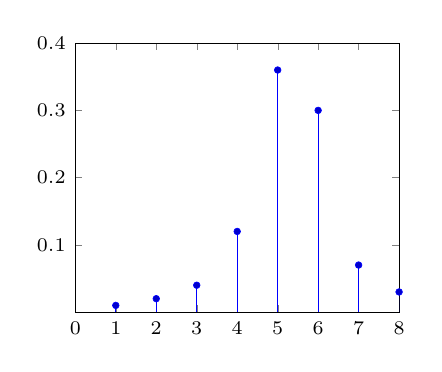
\begin{tikzpicture}[scale = 0.6]
\begin{axis} [
	tick label style={font=\scriptsize, scale = 1/0.6},
    xtick={0,1,...,7,8},
    ytick = {0.1,0.2,0.3,0.4},
    xmin=0, xmax=8,ymin = 0, ymax = 0.4]
\addplot+[ycomb] plot coordinates {(1, 0.01) (2, 0.02) (3, 0.04) (4, 0.12) (5, 0.36) (6, 0.30) (7, 0.07) (8, 0.03) (9, 0.02) (10, 0.01)}; 
\end{axis}
\end{tikzpicture}\qquad\qquad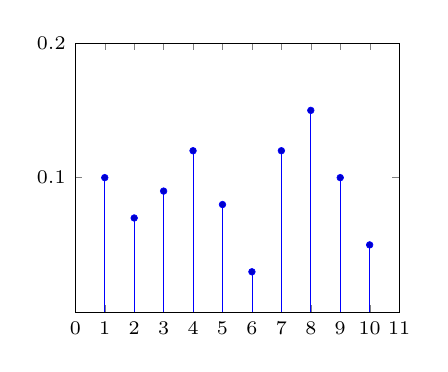
\begin{tikzpicture}[scale = 0.6]
\begin{axis} [
	tick label style={font=\scriptsize, scale = 1/0.6},
    xtick={0,1,...,11},
    ytick = {0.1,0.2},
    xmin=0, xmax=11,ymin = 0, ymax = 0.2]
\addplot+[ycomb] plot coordinates {(1, 0.10) (2, 0.07) (3, 0.09) (4, 0.12) (5, 0.08) (6, 0.03) (7, 0.12) (8, 0.15) (9, 0.1) (10, 0.05)}; 
\end{axis}
\end{tikzpicture}
\end{center}

The values of $X$ tend to be clustered close to the center of the distribution, only very rarely straying under 4 or over 7. On the other hand, $Y$ takes on values far from the center of its distribution quite often. In other words, the distance between the value of $X$ and the center of its distribution is usually smaller than the distance between the value of $Y$ and its center of its distribution. 

In Section \ref{MeasuresOfDispersionSec} we defined the variance of a statistical variable in a dataset as the average squared distance from the mean, and we'll define the variance of a random variance analagously, as the expected squared distance between a random variable and its expected value.

\begin{definition}\index{Random Variable!Variance of}\index{Random Variable!Standard Deviation of}\index{Variance}\index{Standard Deviation}\label{VarianceDefRV} The \newterm{variance} of a discrete random variable $X$ is denoted $\Var(X)$ or $\sigma^{2}_{X}$, and given by 
$$\Var(X) = E[(X - \mu_X)^2] = \sum_{x \in A} (x - \mu_X)^2 f_X(x).$$
The \newterm{standard deviation} of $X$ is then $\sigma_X = \sqrt{\sigma^{2}_X} = \sqrt{\Var(X)}$.
\end{definition}

\begin{remark}
In this section, many expressions are made clearer by using the notation $\mu_X$, or simply $\mu$, in place of $E(X)$, so keep in mind that $\mu_X$ is the expected value of $X$, which is a constant value at the center of the distribution of $X$.
\end{remark}

\begin{example} Determine the expected value, variance, and standard deviation of the random variable $X$ whose pmf is given below.
\renewcommand*{\arraystretch}{1.35}
$$f_X(x) = \left\{
\begin{array}{cl}
      \frac{2}{8} & \text{ if \ } x = 1 \\
			\frac{1}{8} & \text{ if \ } x = 3 \\
			\frac{3}{8} & \text{ if \ } x = 5 \\
			\frac{2}{8} & \text{ if \ } x = 6 \\
      0 & \text{ otherwise} \\ \end{array} 
\right.$$
\renewcommand*{\arraystretch}{1}

First, $E(X) = 1 \cdot \frac{2}{8} + 3 \cdot \frac{1}{8} + 5 \cdot \frac{3}{8} + 6 \cdot \frac{2}{8} = 4$, that is, $\mu_X = 4$. Then we can calculate the variance as
$$\begin{aligned}\Var(X)&=E[(X-\mu_x)^2] \\
&=(1-4)^2 \cdot \frac{2}{8} + (3-4)^2 \cdot \frac{1}{8} + (5-4)^2 \cdot \frac{3}{8} + (6-4)^2 \cdot \frac{2}{8} \\
&=9 \cdot \frac{2}{8} + 1 \cdot \frac{1}{8} + 1 \cdot \frac{3}{8} + 4 \cdot \frac{2}{8} = \frac{30}{8}.\end{aligned}$$

Thus, the standard deviation of $X$ is $\sigma_X = \sqrt{\frac{30}{8}} \approx 1.936$.
\end{example}

\begin{example} In Big Win Bob's game, each player pays $\$1$ to place a bet on a number between 1 and 100, a winning number is selected at random, and the prize for a correct bet is $\$75$. In Conservative Charles' game, each player pays $\$1$ to bet on a number between 1 and 4, a winning number is selected at random, and the prize for a correct bet is $\$3$. Which game would you rather play?

Let $X$ represent a player's net gain in a single play of Bob's game, and let $Y$ represent a player's net gain in a single play of Charles' game.
\eqns{E(X) &= 74 \cdot \frac{1}{100} + (-1) \cdot \frac{99}{100} = -0.25 \\
E(Y) &= 2 \cdot \frac{1}{4} + (-1) \cdot \frac{3}{4} = -0.25}

Thus, it does not matter which game you play in the long run. Over a very large number of plays the games are equivalent, either way the player loses 25\textcent\ per game on average. However, the variances of $X$ and $Y$ are not equal.
\eqns{\Var(X) &= (74 - (-0.25))^2 \cdot \frac{1}{100} + (-1-(-0.25))^2 \cdot \frac{99}{100} \approx 55.69 \\
\Var(Y) &= (2 - (-0.25))^2 \cdot \frac{1}{4} + (-1-(-0.25))^2 \cdot \frac{3}{4} \approx 1.68}

This large difference in the variances indicates Big Win Bob's game is much riskier. In Bob's game players win rarely but win big, while in Charles' game players win small amounts quite often.
\end{example}

Calculating the variance by hand can be tedious, and in practice such calculations are usually done with a computer. It's important to do a few examples by hand though, to understand the subtleties and develop some intuition. In the example above, note that the variance of Big Win Bob's game is dominated by the contribution of the term corresponding to the rare outcome where the player gains \$74, despite the tiny probability, because the difference between the rare \$74 gain and the expected gain is squared.

\begin{example}\label{stdevoneroll}
If $X$ represents the outcome of a single roll of a fair six-sided die, find $\sigma_X$.

First, we compute the mean $E(X) = 1 \cdot \frac{1}{6} + 2 \cdot \frac{1}{6} + 3 \cdot \frac{1}{6} + 4 \cdot \frac{1}{6} + 5 \cdot \frac{1}{6} + 6 \cdot \frac{1}{6} = \frac{7}{2}$. Then we calculate the variance as
$$\begin{aligned}
Var(X) &= \sum_{x \in A} \left(x - \frac{7}{2}\right)^2 \cdot \frac{1}{6} \text{\ , where } A = \{1,2,3,4,5,6\} \\
&= \left(-\frac{5}{2}\right)^2 \cdot \frac{1}{6} + \left(-\frac{3}{2}\right)^2 \cdot \frac{1}{6} + \left(- \frac{1}{2}\right)^2 \cdot \frac{1}{6} + \left(\frac{1}{2}\right)^2 \cdot \frac{1}{6} + \left(\frac{3}{2}\right)^2 \cdot \frac{1}{6} + \left(\frac{5}{2}\right)^2 \cdot \frac{1}{6} \\
&= \frac{25}{24} + \frac{9}{24} + \frac{1}{24} + \frac{1}{24} + \frac{9}{24} + \frac{25}{24} = \frac{35}{12} \\
\end{aligned}$$

The standard deviation is then $\sigma_X = \sqrt{\frac{35}{12}}\approx 1.707$.
\end{example}

\begin{proposition}If $X$ is a discrete random variable with $\Var(X) = 0$, then there is some realization $x$ of $X$ such that $P(X = x) = 1$. That is, $X$ takes a single real value with probability one.
\end{proposition}

\begin{proof}
Suppose there were two different realizations $x_1$ and $x_2$ which both have positive probabilities of occurring. Then at least one of $(x_1 - \mu_X)^2$ and $(x_2 - \mu_X)^2$ is nonzero (since $\mu_X$ cannot be equal to both $x_1$ and $x_2$), but this means at least one of the terms in the sum that defines $E[(X-\mu_X)^2]$ is positive. There are no negative terms in this sum since both squares and probabilities are always non-negative, hence $\Var(X) > 0$.
\end{proof}

\section{The Uniform Distribution}

\begin{definition}\index{Uniform Distribution}\index{Distribution!Uniform}\index{Uniform Distribution} If $X$ is a discrete random variable whose range is an arithmetic progression, and $X$ takes each value with equal probability, we say that $X$ has a \newterm{uniform distribution} on $A$. \end{definition}

\begin{example} Suppose that $X$ represents the result of a single fair die roll, then $X$ is uniformly distributed on $A = \{1,2,3,4,5,6\}$, since $P(X = x) = \frac{1}{6}$ for all $x \in A$.
\end{example}

The notation $X \sim \Uniform(n)$ indicates $X$ is a discrete random variable which is uniformly distributed on $A = \{1,2,3, \, .. \,, n\}$. We could write $X \sim \Uniform(6)$ to describe the distribution of the random variable in the example of a die roll above. 

If $X$ is uniformly distributed on the set $A$, then its pmf has the form
$$f_X(x) = \left\{
\renewcommand*{\arraystretch}{1.35}
\begin{array}{cl}
      \frac{1}{n} & \text{ if \ } x \in A \\
      0 & \text{ otherwise} \\ \end{array},
      \renewcommand*{\arraystretch}{1}
\right.$$
which yields a lollipop plot with a finite number lollipops of the equal height, spaced evenly along the horizontal axis. For example, the lollipop plot below shows the pmf of a random variable uniformly distributed on $A = \{-1,0,1,2\}$.

\begin{center}
\begin{tikzpicture}[scale = 0.6]
\begin{axis} [
	tick label style={font=\scriptsize, scale = 1/0.6},
    xtick={-2,-1,...,3},
    ytick = {0.1,0.2,0.3},
    xmin=-2, xmax=3,ymin = 0, ymax = 0.3]
\addplot+[ycomb] plot coordinates {(-1, 0.25) (0, 0.25) (1, 0.25) (2, 0.25)}; 
\end{axis}
\end{tikzpicture}
\end{center}

The expected value of a uniformly distributed variable on the set $A$ is simply the average of the values in $A$. Formally, if $X$ is uniformly distributed on the set $A = \{a_1, a_2,\, \dots \, , a_n\}$, then
$$E(X) = a_1 \cdot \textstyle\frac{1}{n} + a_2 \cdot \frac{1}{n} + \cdots + a_n \cdot \frac{1}{n} = \frac{a_1 + a_2 + \dots + a_n}{n}.$$
In particular, if $X \sim \Uniform(n)$, then $E(X) = \frac{1+2+3+\cdots+n}{n} = \frac{\frac{n(n+1)}{2}}{n} = \frac{n+1}{2}$.

\begin{remark}
When an element is being chosen from a set, and each element in that set has the same probability of being selected, we say the choice is made \emx{uniformly at random}.
 
One could `randomly' select a number from the set $A = \{0,1,2,3\}$ by flipping a coin three times and counting the number of heads, but not all outcomes would be equally likely. Typically when an author uses the words `at random' in mathematics, what's meant is that each possible outcome is equally likely, not that the outcome is the result of some unspecified random process. To be as clear as possible, it's good practice to use the term \emx{uniformly}.
\end{remark}

\section{The Bernoulli Distribution}\label{BernoulliDist}

Suppose that we perform an experiment with only two possible outcomes, usually called success and failure, and the probability of success is known to be $p$. Such an experiment is called a Bernoulli trial, after the mathematician Jacob Bernoulli. If $X$ is a random variable that counts the number of successes in a single Bernoulli trial (either zero or one), we say $X$ has a Bernoulli distribution with parameter $p$.

\begin{definition}\index{Bernoulli Distribution}\index{Distribution!Bernoulli}The random variable $X$ has a \newterm{Bernoulli distribution} with parameter $p$, written $X \sim \Bernoulli(p)$, if
$$f_X(x) = \left\{
\renewcommand*{\arraystretch}{1.35}
\begin{array}{cl}
      p & \text{ if \ } x =1 \\
      1-p & \text{ if \ } x =0 \\ 
      0 & \text{ otherwise} \\ \end{array}.
      \renewcommand*{\arraystretch}{1}
\right.$$

In other words, $X$ takes the value $1$ with probability $p$, and $0$ with probability $1-p$.
\end{definition}

Think of a Bernoulli random variable as counting the number of heads observed in a single flip of a coin with a given bias. If $X$ represents the number of heads in a single flip of a fair coin, then $X \sim \Bernoulli(0.5)$, and if $Y$ represents the number of heads in a single flip of a biased coin which lands on heads only $30\%$ of the time, then $Y \sim \Bernoulli(0.3)$. The pmf of $Y$ is graphed below.

\begin{center}
\begin{tikzpicture}[scale = 0.6]
\begin{axis} [
	tick label style={font=\scriptsize, scale = 1/0.6},
    xtick={0,1},
    ytick = {0.3,0.6,0.9},
    xmin=-0.5, xmax=1.5, ymin = 0, ymax = 0.9]
\addplot+[ycomb] plot coordinates {(0, 0.7) (1, 0.3)}; 
\end{axis}
\end{tikzpicture}
\end{center}

\begin{proposition}\label{BernoulliExpectation}\index{Bernoulli Distribution!Expected Value of}\index{Bernoulli Distribution!Variance of} If $X \sim \Bernoulli(p)$, then $E(X) = p$ and $\Var(X) = p(1-p)$.
\end{proposition}

\begin{proof} These results both follow from direct calculations. From the probability mass function above we have $E(X) = 0 \cdot (1-p) + 1 \cdot p  = p$. We can then calculate
$$\begin{aligned}\Var(X) &= E[(X - \mu_X)^2] = E[(X - p)^2] = (0-p)^2 \cdot (1-p) + (1-p)^2 \cdot p \\
&= p^2(1-p) + (1-p)^2p = p(1-p)(p+(1-p)) = p(1-p).\end{aligned}$$
\end{proof}

Bernoulli random variables are simple but fundamental in probability and statistics. The Binomial, Geometric, and Poisson distributions, all of which come up frequently in scientific practice, can be defined in terms of Bernoulli random variables. In this course, we'll cover only the Binomial distribution, the others are studied in the Probability \& Random Variables option course, 201-PRV.

\section{The Binomial Distribution}

Suppose we perform a fixed number of Bernoulli trials (call this number $n$). Each trial has the same probability of success (call this value $p$), and the results of the $n$ consecutive trials form a sequence of independent Bernoulli random variables. If $X$ counts the total number of successes after all the trials have been performed, then we say that $X$ has a Binomial distribution.

\begin{definition}\index{Binomial Distribution}\index{Distribution!Binomial} The random variable $X$ has a \newterm{binomial distribution} with parameters $n$ and $p$, written $X \sim \Binomial(n,p)$, if
$$f_X(x) = \left\{
\renewcommand*{\arraystretch}{1.35}
\begin{array}{cl}
      \displaystyle\binom{n}{x}(p)^x(1-p)^{n-x} & \text{ if \ } x = 0, 1, 2, \dots \, , n \\
      0 & \text{ otherwise } \\ \end{array}.
      \renewcommand*{\arraystretch}{1}
\right.$$
\end{definition}

Below on the left is the pmf of a binomial distribution with $n = 5$, $p = 0.5$, and on the right, the pmf of a binomial distribution with $n = 9$, $p = 0.85$.

\begin{center}
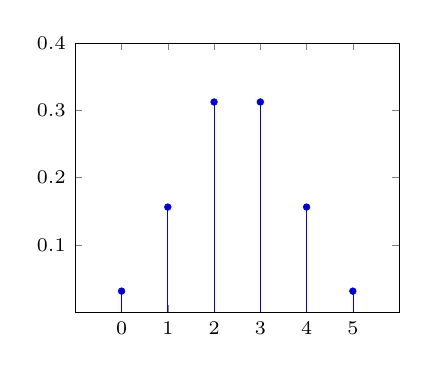
\begin{tikzpicture}[scale = 0.6]
\begin{axis} [
	tick label style={font=\scriptsize, scale = 1/0.6},
    xtick={0,1,...,5},
    ytick = {0.1,0.2,0.3,0.4},
    xmin=-1, xmax=6, ymin = 0, ymax = 0.4]
\addplot+[ycomb] plot coordinates {(0, 0.03125) (1, 0.15625) (2, 0.3125) (3, 0.3125) (4, 0.15625) (5, 0.03125)}; 
\end{axis}
\end{tikzpicture} \qquad\qquad  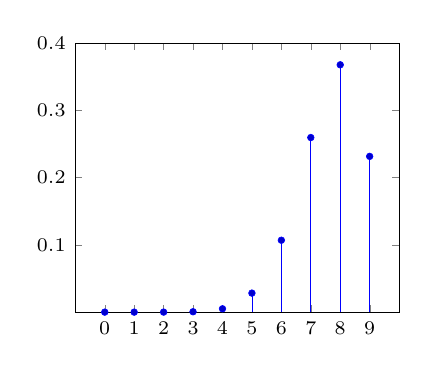
\begin{tikzpicture}[scale = 0.6]
\begin{axis} [
	tick label style={font=\scriptsize, scale = 1/0.6},
    xtick={0,1,...,9},
    ytick = {0.1,0.2,0.3,0.4},
    xmin=-1, xmax=10, ymin = 0, ymax = 0.4]
\addplot+[ycomb] plot coordinates {(0, 0.00000003) (1, 0.000002) (2, 0.000045) (3, 0.00058) (4,0.005) (5, 0.0283) (6, 0.10692) (7,0.2596) (8,0.3678) (9,0.2316)}; 
\end{axis}
\end{tikzpicture}
\end{center}

To derive this probability mass function, imagine recording of the results of the Bernoulli trials as an $n$ letter long sequence of $S$'s and $F$'s, representing success and failure respectively. By the Mississippi formula from Section \ref{PermutationsSec}, the number of such sequences in which $x$ successes occur is $\frac{n!}{x!(n-x)!} = \binom{n}{x}$.

Consider any such sequence, say $SFSSSFF$ for example. Here $n=7$, and $x=4$ successes occurred. The probability this particular ordered sequence occurs is not hard to calculate since we're performing independent Bernoulli trials, each with the same probability of success. Every $S$ occurs with probability $p$, and every $F$ with probability $1-p$. There are four $S$'s and three $F$'s, and the trials are independent, so this sequence occurs with probability $p^4(1-p)^3$.

In total then, there are $\binom{n}{x}$ sequences of outcomes with $x$ successes, and each sequence occurs with probability $p^x(1-p)^{n-x}$, so $P(X = x) = \binom{n}{x}p^x(1-p)^{n-x}$.

The number of heads in $n$ flips of a coin is the example that should immediately come to mind when you think of a binomial distribution, but binomial distributions also appear in many practical contexts involving samples.

\begin{example}Suppose that in a certain country's election, $56\%$ of the voting population will vote for a particular candidate, Bob. If you select seven members of the voting population uniformly at random, and ask them who they'll vote for (assume they'll answer honestly), what is the probability your poll will incorrectly conclude that Bob will win less than half the vote?

Let $X$ represent the number of people who respond by saying that they'll vote for Bob. If we regard such a response as a success, and each interview is done without knowledge of the results of any of the others, then $X \sim \Binomial(7, 0.56)$.

The result we're seeking is the probability that there are fewer than four successes, which we calculate from the pmf as follows.
$$\begin{aligned}P(X \leq 3) &= \sum_{i=0}^{3} P(X = i) = \sum_{i=0}^{3} \binom{7}{i}(0.56)^{i}(0.44)^{7-i} \\
&\approx 0.0032 + 0.0284 + 0.1086 + 0.2304 \\
&= 0.3706 \approx 37\%\end{aligned}$$

There is a $37\%$ chance that the results of this poll will incorrectly predict that Bob will not win a majority of the vote.
\end{example}

\begin{remark}
It would be easier to use the cdf to evaluate $P(X \leq 3)$, but unfortunately, the cdf for a binomial distribution does not have a simple closed form, so we're stuck summing the values of the pmf.
\end{remark}

One of the reasons the binomial distribution appears in many contexts is that the process of evaluating a claim by doing repeated independent trials, which could be interviews, simulations, or literal laboratory experiments, is such a fundamental practice.

\begin{theorem}\index{Binomial Distribution!Expected value of}\index{Binomial Distribution!Variance of}If $X \sim \Binomial(n,p)$, then $E(X) = np$ and $\Var(X) = np(1-p)$.
\end{theorem}

These formulas follow from properties of expected value and sums of random variables which are not covered in this course, but appear in the Probability \& Random Variables option course, 201-PRV.

\begin{example} Let $X$ be the number of doubles in five rolls of a pair of dice, and let $Y$ be the number of heads in three flips of a fair coin. Which quantity is larger on average? Which quantity is more variable?

$X$ is a binomial random variable with $n = 5$ and $p = \frac{6}{36} = \frac{1}{6}$, so $E(X) = np = \frac{5}{6}$ and $\Var(X) = np(1-p) = 5(\frac{1}{6})(\frac{5}{6}) = 25/36 \approx 0.694$.

$Y$ is a binomial random variable with $n = 3$ and $p = \frac{1}{2}$, so $E(Y) = np = \frac{3}{2}$ and $\Var(X) = np(1-p) = 3(\frac{1}{2})(\frac{1}{2}) = 3/4 \approx 0.75$.

Therefore, $Y$ is larger on average. The second question is somewhat ambiguous, but if we use the variance as our measure of variability, $Y$ is a little more variable then $X$.
\end{example}

\begin{example}
Edward lives in a country with an unreliable mail system, where 7\% of parcels do not make it to their destination. He wants to send two books to his brother, each with a value of \$20. If he sends them in one parcel, the postage is \$5.20, and if he sends them separately, the postage is \$3.30 for each book. To minimize his expected losses, which method is preferable?

Let $X \sim \Bernoulli(0.07)$, then sending both books in one parcel, the \$5.20 postage charge always applies, and \$40 is lost if $X = 1$. If $L$ represents Edward's loss, then $L = 5.20 + 40X$, and therefore $E(L) = 5.20 + 40E(X) = 5.20 + 40 \cdot 0.07 = 8$.

If the two books are each sent separately, then $L = 6.60 + 20Y$, where $Y \sim \Binomial(2,0.07)$. Thus, $E(L) = 6.60 + 20E(Y) = 6.60 + 20 \cdot 2 \cdot 0.07 = 9.4$, so sending both books in one package is the option with the smaller expected loss.
\end{example}

\section{Continuous Random Variables}\label{ContinuousRVSection}

In Section \ref{RVIntroSec}, we defined a random variable as a function from $\Omega$ to $\mathbb{R}$, but have so far only considered random variables that take values in some countable subset $A \subseteq \mathbb{R}$. We saw that we could specify the distribution of such a random variable using a probability mass function, or a cumulative distribution function.

Our goal is now to understand what happens when a random variable can take any value in some interval $I \in \mathbb{R}$. Consider for example a random variable $X$ which represents a number chosen uniformly at random from the interval $[0,1]$. Unfortunately, it's not possible to express the distribution of $X$ as a table, since $[0,1]$ is not a countable set, so we can't list its values one-by-one.

Fortunately, the cumulative distribution function comes to the rescue. What is $P(X \leq \frac{2}{3})$? If we divide the interval into thirds, then $X \leq \frac{2}{3}$ when $X$ falls into one of the left two thirds, which should happen two thirds of the time if $X$ is equally likely to fall anywhere in $[0,1]$.
\begin{center}
\begin{tikzpicture}
\draw (0,0) -- (3,0);
\draw[shift={(0,0)},color=black] (0pt,3pt) -- (0pt,-3pt);
\draw[shift={(3,0)},color=black] (0pt,3pt) -- (0pt,-3pt);
\foreach \x in {1,2}
\draw[shift={(\x,0)},color=black] (0pt,0pt) -- (0pt,-3pt) node[below] 
{\small$\frac{\x}{3}$};
\draw (0,-0.2) node[below]{\small$0$};
\draw (3,-0.2) node[below]{\small$1$};
\fill [pattern=north west lines, pattern color=black] (0,0.1)--(2,0.1)--(2,-0.1)--(0,-0.1);
\end{tikzpicture}
\end{center}

Thus, $P(X \leq \frac{2}{3}) = \frac{2}{3}$. By a similar argument, it should be clear that $P(X \leq x) = x$ for any $x \in [0,1]$ and therefore, the cumulative distribution function of $X$ is the function given below.

\begin{center}
    \begin{minipage}{0.5\textwidth}
        \centering
        \renewcommand*{\arraystretch}{1.35}
$$F_X(x) = \left\{
\begin{array}{cl}
      0 & \text{ if \ } x < 0  \\
      x & \text{ if \ } 0 \leq x < 1  \\
      1 & \text{ if \ } x \geq 1 \\ \end{array}
\right.$$
\vspace{0.75em}
\renewcommand*{\arraystretch}{1}
    \end{minipage}%
    \begin{minipage}{0.5\textwidth}
        \centering
    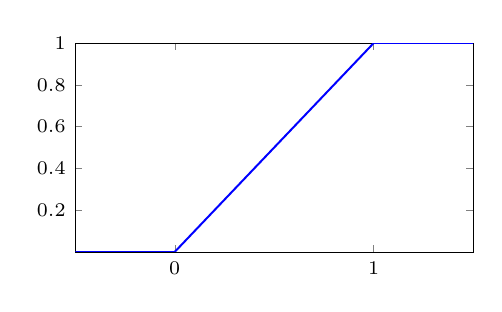
\begin{tikzpicture}[scale = 0.6]
       \begin{axis}[
       tick label style={font=\scriptsize, scale = 1/0.6},
    xtick={0,1},
    ytick = {0.2,0.4,...,1},
    xmin=-0.5, xmax=1.5, ymin = 0, ymax = 1, width=10cm, height=6cm]
       \addplot[very thick,domain=-1:0,blue] {0};
       \addplot[very thick,domain=0:1,blue] {x};
       \addplot[very thick,domain=1:2,blue] {1};
    \end{axis}
\end{tikzpicture}
\end{minipage}
\end{center}
%unit vector ratio=1 1 1, ymin=-0.0025,ymax=1.0025,xmin=-0.5, xmax = 1.5, xtick={0,1},ytick={0,0.2,0.4,0.6,0.8,1}

Using this cdf, we can determine the probability that $X$ will be in various subsets of $[0,1]$. Let's take the interval $(\frac{2}{5},\frac{2}{3})$. Using the cdf above, we can compute

\begin{center}
    \begin{minipage}{0.5\textwidth}
        \centering
        $$\begin{aligned}P(X \in (\textstyle\frac{2}{5},\frac{2}{3})) &= P(\textstyle\frac{2}{5} < X < \frac{2}{3}) \\
&= P(X < \textstyle\frac{2}{3}) - P(X \leq \frac{2}{5}) \\
&= F_X(\textstyle\frac{2}{3} - ) - F_X(\frac{2}{5}) \\
&= \textstyle \frac{2}{3} - \frac{2}{5} = \frac{4}{15}\end{aligned}$$
\vspace{0.25em}
    \end{minipage}%
    \begin{minipage}{0.5\textwidth}
        \centering
    \begin{tikzpicture}[scale = 0.6]
       \begin{axis}[tick label style={font=\scriptsize, scale = 1/0.6},
    xtick={0,2/5,2/3,1},
    xticklabels={$0$,$\frac{2}{5}$,$\frac{2}{3}$,$1$},
    ytick = {0.2,0.4,...,1},
    xmin=-0.5, xmax=1.5, ymin = 0, ymax = 1, width=10cm, height=6cm]
       \addplot[very thick,domain=-1:0,blue] {0};
       \addplot[name path = f, very thick,domain=0:1,blue] {x};
       \addplot[very thick,domain=1:2,blue] {1};
       \draw[black] (axis cs: 2/3,0) -- (axis cs: 2/3,2/3);
       \draw[black] (axis cs: 2/5,0) -- (axis cs: 2/5,2/5);
    \end{axis}
\end{tikzpicture}
\end{minipage}
\end{center}


\begin{keypoint}
If the cdf of $X$ is continuous, then $\lim_{x \to a^{-}}F_X(x) = \lim_{x \to a^{+}}F_X(x) = F_X(a)$, and hence $F_X(a-)$, $F_X(a+)$ and $F_X(a)$ are all equal. This implies a random variable $X$ with a continuous cdf will take any fixed realization with probability zero, since
$$P(X = x) = P(X \leq x) - P(X < x) = F_X(x) - F_X(x-) = 0.$$

Furthermore, $P(X \in (a,b))$, $P(X \in [a,b))$, $P(X \in (a,b])$, and $P(X \in [a,b])$ are all equal to $F_X(b) - F_X(a)$. Including or excluding endpoints makes no difference.
\end{keypoint}

\begin{definition}
If $X$ is a random variable whose cumulative distribution function $F_X(x) = P(X \leq x)$ is continuous, then we say $X$ is a \newterm{continuous random variable}\index{Continuous Random Variable}.
\end{definition}

\begin{example}\label{ContinuousCDFExample} Let X be a random variable with cdf given below. Find $P(X \in (\frac{1}{3}, 1) \cup [\frac{3}{2}, \frac{5}{2}])$.
\vspace{-1em}
\begin{center}
    \begin{minipage}{.5\textwidth}
        \centering
        \renewcommand*{\arraystretch}{1.35}
\eqns{F_X(x) = \left\{
\begin{array}{cl}
      0 & \text{ if \ } x < 0  \\
      \frac{1}{2}x & \text{ if \ } 0 \leq x < 1  \\
      \frac{1}{2} & \text{ if \ } 1 \leq x < 2 \\ 
      x - \frac{3}{2} & \text{ if \ } 2 \leq x < \frac{5}{2} \\ 
      1 & \text{ if \ } x \geq \frac{5}{2} \\ \end{array}
\right.}
\vspace{1.25em}
\renewcommand*{\arraystretch}{1}
    \end{minipage}%
    \begin{minipage}{0.5\textwidth}
        \centering
    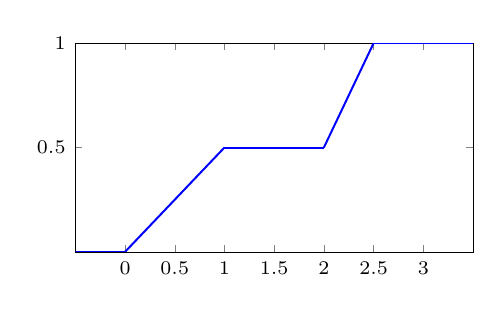
\begin{tikzpicture}[scale = 0.6]
       \begin{axis}[tick label style={font=\scriptsize, scale = 1/0.6},
    xtick={0,0.5,...,3},
    ytick = {0.5,1},
    xmin=-0.5, xmax=3.5, ymin = 0, ymax = 1, width=10cm, height=6cm]
       \addplot[very thick,domain=-1:0,blue] {0};
       \addplot[very thick,domain=0:1,blue] {0.5*x};
       \addplot[very thick,domain=1:2,blue] {0.5};
       \addplot[very thick,domain=2:2.5,blue] {x -1.5};
       \addplot[very thick,domain=2.5:3.5,blue] {1};
    \end{axis}
\end{tikzpicture}
\end{minipage}
\end{center}

Since the events $X \in (\frac{1}{3}, 1)$ and $X \in [\frac{3}{2}, \frac{5}{2}]$ are mutually exclusive,
$$\begin{aligned}P(X \in (\textstyle\frac{1}{3}, 1) \cup [\frac{3}{2},\frac{5}{2}]) &= P(X \in (\textstyle\frac{1}{3}, 1)) + P(X \in [\frac{3}{2},\frac{5}{2}]) \\
%&= P(X < 1) - P(X \leq \textstyle\frac{1}{3}) + P(X \leq  \frac{5}{2}) - P(X < \frac{3}{2}) \\
&= F_X(1) - F_X(\textstyle\frac{1}{3}) + F_X( \frac{5}{2}) - F_X(\frac{3}{2}) \\
&= \textstyle\frac{1}{2} - \frac{1}{2}\cdot\frac{1}{3} + 1 - \frac{1}{2} \\
&= \textstyle\frac{1}{2} - \frac{1}{6} + 1 - \frac{1}{2} = \frac{5}{6}.\end{aligned}$$
\end{example}

\subsection*{Probability Density Functions}
Consider a continuous random variable $X$, and two real numbers $r$ and $s$. We now know that $P(X = r)$ and $P(X = s)$ are both zero, but we can still ask whether $X$ is more likely to end up close to $r$ or close to $s$.

We can formalize this by asking for the probability $X$ lies in each of the tiny intervals $(s-\epsilon,\, s + \epsilon)$ and $(r-\epsilon, \,r+ \epsilon)$, for some very small positive number $\epsilon$. Take for instance the random variable $X$ in Example \ref{ContinuousCDFExample} above. Is it more likely this variable takes a value close to $\frac{1}{2}$, or a value close to $\frac{9}{4}$?

\begin{center}
\begin{tikzpicture}[scale = 0.6]
       \begin{axis}[tick label style={font=\scriptsize, scale = 1/0.6},
    xtick={1/2,9/4},
    xticklabels={\small$\frac{3}{2}$,\small$\frac{9}{4}$},
    ytick = {0.5,1},
    xmin=-0.5, xmax=3.5, ymin = 0, ymax = 1, width=12cm, height=8cm]
       \addplot[very thick,domain=-1:0,blue] {0};
       \addplot[very thick,domain=0:0.38,blue] {0.5*x};
       \addplot[very thick,domain=0.38:0.62,red] {0.5*x};
       \addplot[very thick,domain=0.62:1,blue] {0.5*x};
       \addplot[very thick,domain=1:2,blue] {0.5};
       \addplot[very thick,domain=2:2.13,blue] {x -1.5};
       \addplot[very thick,domain=2.13:2.37,red] {x -1.5};
       \addplot[very thick,domain=2.37:2.5,blue] {x -1.5};
       \addplot[very thick,domain=2.5:3.5,blue] {1};
       \node[label={},circle,fill,inner sep=1pt,red] at (axis cs:0.38,0.19) {};
       \node[label={},circle,fill,inner sep=1pt,red] at (axis cs:0.62,0.31) {};
       \node[label={},circle,fill,inner sep=1pt,red] at (axis cs:2.13,0.63) {};
       \node[label={},circle,fill,inner sep=1pt,red] at (axis cs:2.37,0.87) {};
    \end{axis}
    \draw[thick,red] (2.9,0) node {\small )};
    \draw[thick,red] (2.3,0) node {\small (};
    \draw[red,thick] (2.3,0)  -- (2.9,0);
    \draw[thick,red] (7.45,0) node {\small )};
    \draw[thick,red] (6.85,0) node {\small (};
    \draw[red,thick] (7.45,0)  -- (6.85,0);
\end{tikzpicture}
\end{center}

The probability $X$ lies in the interval $(a,b)$ is $F_X(b) - F_X(a)$, the difference in the value of the cdf at the endpoints. For the cdf shown above, the graph is twice as steep when it's near $\frac{9}{4}$ than it is when it's near $\frac{1}{2}$, and hence this difference is twice as large. Therefore, $X$ is twice as likely to assume values near $\frac{9}{4}$ than it is to assume values near $\frac{1}{2}$.

In general then, the probability $X$ lies close to a given value is proportional to the slope of the cdf at that value. But we know how to measure the slope of any function, with the derivative. Thus, given any $x \in \mathbb{R}$, if we evaluate the derivative of $F_X$ at $x$, the larger the result, the more likely it is that $X$ takes a value very close to $x$. Remember that the probability $X=x$ must be zero for all $x \in \mathbb{R}$, so when we evaluate the derivative of $F_X$ at $x$, the result is not a probability, instead it's known as a probability density, and the derivative of $F_X$ is called the probability density function of $X$. 

\begin{definition}\index{Probability Density Function}\index{Probability Density}If $X$ is a continuous random variable with cdf $F_X$, the \newterm{probability density function} of $X$ is denoted $f_X$ and is defined by $f_X(x) = \frac{d}{dx}{F_X}(x)$.
\end{definition}

The cdf $F_X$ of the continuous random variable $X$ defined in Example \ref{ContinuousCDFExample} above is shown once again on the left, and the corresponding probability density function $f_X$ is on the right. It's standard practice to draw vertical lines on the graph of the probability density function as below. These lines are technically not part of the graph (they are jump discontinuities), but make for a more appealing image.

\begin{center}
    \begin{minipage}{.5\textwidth}
        \centering
       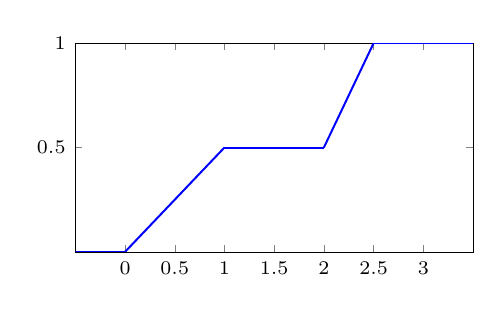
\begin{tikzpicture}[scale = 0.6]
       \begin{axis}[tick label style={font=\scriptsize, scale = 1/0.6},
    xtick={0,0.5,...,3},
    ytick = {0.5,1},
    xmin=-0.5, xmax=3.5, ymin = 0, ymax = 1, width=10cm, height=6cm]
       \addplot[very thick,domain=-1:0,blue] {0};
       \addplot[very thick,domain=0:1,blue] {0.5*x};
       \addplot[very thick,domain=1:2,blue] {0.5};
       \addplot[very thick,domain=2:2.5,blue] {x -1.5};
       \addplot[very thick,domain=2.5:3.5,blue] {1};
    \end{axis}
\end{tikzpicture}
    \end{minipage}%
    \begin{minipage}{0.5\textwidth}
        \centering
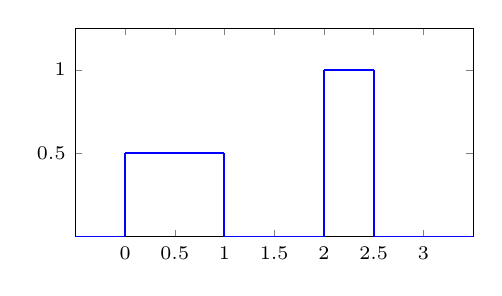
\begin{tikzpicture}[scale = 0.6]
       \begin{axis}[tick label style={font=\scriptsize, scale = 1/0.6},
    xtick={0,0.5,...,3},
    ytick = {0.5,1},
    xmin=-0.5, xmax=3.5, ymin = 0, ymax = 1.25, width=10cm, height=6cm]
       \addplot[very thick,domain=-1:0,blue] {0};
       \addplot[very thick,domain=0:1,blue] {0.5};
       \addplot[very thick,domain=1:2,blue] {0};
       \addplot[very thick,domain=2:2.5,blue] {1};
       \addplot[very thick,domain=2.5:3.5,blue] {0};
       \draw[very thick, blue, -] (axis cs:0,0) -- (axis cs:0,0.5);
       \draw[very thick, blue, -] (axis cs:1,0) -- (axis cs:1,0.5);
       \draw[very thick, blue, -] (axis cs:2,0) -- (axis cs:2,1);
       \draw[very thick, blue, -] (axis cs:2.5,0) -- (axis cs:2.5,1);
    \end{axis}
    \end{tikzpicture}
\end{minipage}
\end{center}

We'll often use pdf to abbreviate probability density function. The rationale for the term `probability density' is the following: when considering a rod of metal or other material, we can only ask for the mass of a contiguous piece of the material, since the mass at a point is always zero. We can, however, consider the density of the material to be well defined at a point, as the rate of change in mass at that point as we move along the rod. The situation with continuous random variables is analogous: a probability density measures the rate of change of the cdf as we move along it, in other words, the rate at which probability is accumulating as we move past that point.

\begin{proposition}If $X$ is a continuous random variable, then the probability $X$ lies in the interval $(a,b)$ is the area under $f_X$ on $(a,b)$.
\end{proposition}

\begin{proof} Calculating $P(X \in (a,b))$ using the cdf $F_X$ as we have done in the examples above, and applying the fundamental theorem of calculus, we have
$$P(X \in (a,b)) = F_X(b) - F_X(a) = \int_{a}^{b} \frac{d}{dx} F_X(x) \, dx = \int_{a}^{b} f_X(x) \, dx.$$
This integral is the area under $f_X$ on $(a,b)$. Note that the result would be the same with any of the intervals $(a,b]$, $[a,b)$, or $[a,b]$. \end{proof}

\begin{example} Let X be the continuous random variable whose pdf is given below. Find $P(X > \frac{3}{2})$.

\begin{center}
    \begin{minipage}{.5\textwidth}
        \centering
        \renewcommand*{\arraystretch}{1.35}
\eqns{f_X(x) = \left\{
\begin{array}{cl}
      \frac{2}{x^2} & \text{ if \ } 1 \leq x \leq 2  \\
      0 & \text{ otherwise \ }  \\ \end{array}
\right.}
\vspace{1.25em}
\renewcommand*{\arraystretch}{1}
    \end{minipage}%
    \begin{minipage}{0.5\textwidth}
        \centering
    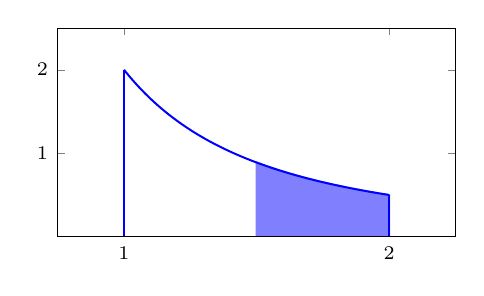
\begin{tikzpicture}[scale =0.6]
       \begin{axis}[tick label style={font=\scriptsize, scale = 1/0.6},
    	xtick={1,2},
    	ytick = {1,2},
    	xmin=0.75, xmax=2.25, ymin = 0, ymax = 2.5, width=10cm, height=6cm]
        \addplot[fill = blue, very thick,domain=1.5:2,blue!50, samples=100] {2/(x*x)}\closedcycle;
       \addplot[very thick,domain=1:2,blue, samples=100] {2/(x*x)};
       \draw[very thick, blue, -] (axis cs:1,2) -- (axis cs:1,0);
       \draw[very thick, blue, -] (axis cs:2,0.5) -- (axis cs:2,0);
       \addplot[domain=-3:3] {0};
    \end{axis}
\end{tikzpicture}
\end{minipage}
\end{center}

$$P(X > \textstyle\frac{3}{2}) = \displaystyle\int_{\frac{3}{2}}^{2} f_X(x) \, dx = \int_{\frac{3}{2}}^{2} \frac{2}{x^2} \, dx =  \left.-\frac{2}{x}\,\right|_{\frac{3}{2}}^{2} = -\frac{2}{2} - \left(- \frac{2}{\frac{3}{2}}\right) = \frac{1}{3}$$
\end{example}

\begin{keypoint}
The area above the interval $I$ under the probability density function $f_X$ is the probability $X$ takes a value in $I$. This is why the probability density function is so useful. It gives a representation of the distribution of a continuous random variable which is as geometrically intuitive as a histogram, and allows us to apply the tools of calculus directly to compute probabilities.
\end{keypoint}

\begin{proposition}If $X$ is any continuous random variable with cdf $F_X$, the pdf $f_X$ satisfies each of the properties below.
\vspace{-0.25em}
\begin{enumerate}
\item For all $x \in \mathbb{R}$, $f_X(x) \geq 0$.
\item $\int_{-\infty}^{\infty} f_X(x) \, dx = P(-\infty < X < \infty) = 1$.
\item $\int_{-\infty}^{t} f_X(x) \, dx = P(X \leq t) = F_X(t)$.
\end{enumerate}
\end{proposition}

Informally, every non-negative function which encloses an area of one between its graph and the horizontal axis is the pdf of some continuous random variable, the cdf of which can be recovered through integration, as in the third property above.

\begin{example}Consider the function $f$ given below. Find $c$ so that this function is the pdf of some continuous random variable.
\renewcommand*{\arraystretch}{1.35}
\eqns{f(x) = \left\{
\begin{array}{cl}
      cxe^{-x} & \text{ if \ } x > 0  \\
      0 & \text{ otherwise \ }  \\ \end{array}
\right.}
\renewcommand*{\arraystretch}{1}

Since $e^{x}>0$ always, we have $xe^{-x} > 0$ when $x > 0$, and thus $f$ is non-negative when $c > 0$. We must find a positive value for $c$ such that the area under $f$ is one, so we evaluate the area under $f$.
$$\int_{-\infty}^{\infty} f(x) \, dx = \int_{0}^{\infty} cxe^{-x} \, dx =c \int_{0}^{\infty} xe^{-x} \, dx =  c(-x-1)e^{-x} \biggr|_{0}^{\infty}$$

The last equality comes from using integration by parts. To complete the evaluation, we can use L'H\^{o}pital's rule.
$$\begin{aligned}c(-x-1)e^{-x} \biggr|_{0}^{\infty} &= \lim_{x \to \infty} \left(c(-x-1)e^{-x}\right) - c(-0-1)e^{0}\\
&= c \lim_{x \to \infty} \left( \textstyle\frac{-x-1}{e^{x}}\right) + c \\
&\stackrel{H}{=} c \lim_{x \to \infty} \left( \textstyle\frac{-1}{e^{x}}\right) + c \\
&= 0 + c = c\end{aligned}$$

The area under $f$ is simply $c$, and therefore if we take $c=1$, $f$ is a pdf. The graph of $f$ with $c = 1$ is given below.
\begin{center}
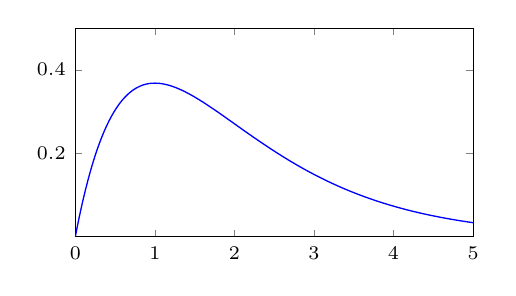
\begin{tikzpicture}[scale=0.6]
       \begin{axis}[tick label style={font=\scriptsize, scale = 1/0.6},
    	xtick={0,1,...,5},
    	ytick = {0.2,0.4},
    	xmin=0, xmax=5, ymin = 0, ymax = 0.5, width=10cm, height=6cm]
       \addplot[thick,domain=0:5,blue, samples = 200] {x*(e^(-x))};
    \end{axis}
\end{tikzpicture}
\end{center}
\end{example}

As you can see, the material that was covered in Calculus I \& II will be very relevant in the world of continuous random variables. If you're a bit rusty, don't be worried. Using the tools of calculus to work with general continuous random variables is a topic we'll not go into in this course, and instead leave for the Probability \& Random Variables option course, 201-PRV. It's also worth noting that the integrals appearing in problems involving continuous random variables are often either very simple, or not possible to evaluate using the methods of elementary calculus (we'll see an example in the next section). The example above was created specifically to remind you about integration by parts and L'H\^{o}pital's rule.

\subsection*{Expectation for Continuous Random Variables}

The expected value of a continuous random variable $X$ is defined in essentially the same way the expected value of a discrete random variable, but in place of a probability mass function we have a probability density function, and in place of a sum we have the continuous analogue, an integral.

\begin{definition}\index{Expected Value}\index{Expected Value! of a Continuous R.V.}
If $X$ is a continuous random variable, the expected value of $X$ is denoted $E(X)$ or $\mu_X$, and defined by
$$E(X) = \int_{-\infty}^{\infty}x f_X(x) \, dx.$$

Note that this improper integral may not converge, in which case the expected value is undefined.
\end{definition}

\begin{example}
Find the expected value of the random variable $X$ whose pdf is given by $f_X(x) = 2/x^2$ on $[1,2]$.
$$E(X) = \int_{-\infty}^{\infty}x f_X(x) \, dx = \int_{1}^{2}x \,\frac{2}{x^2} \, dx = 2\int_{1}^{2}\frac{1}{x}\, dx = 2 \ln(x) \bigr|_{1}^{2} = 2\ln(2)$$
\end{example}

\begin{example}\label{CauchyExpectation}
Consider the random variable $X$ whose pdf is given below. Show $E(X)$ is undefined.
\begin{center}
    \begin{minipage}{.5\textwidth}
        \centering
\eqns{f_X(x) = \frac{1}{\pi(1+x^2)}\text{\ \ on \ }(-\infty,\infty)}
\vspace{1.25em}
    \end{minipage}%
    \begin{minipage}{0.5\textwidth}
        \centering
    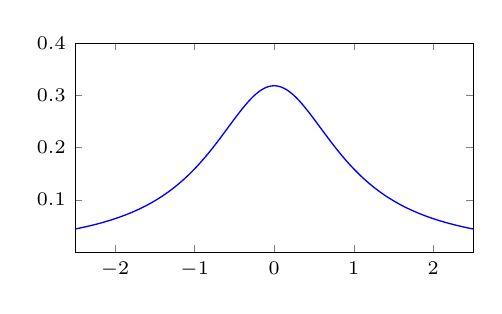
\begin{tikzpicture}[scale=0.6]
       \begin{axis}[tick label style={font=\scriptsize, scale = 1/0.6},
    xtick={-2,-1,...,2},
    ytick = {0.1,0.2,0.3,0.4},
    ymin=0,ymax=0.4,xmin=-2.5, xmax = 2.5, width=10cm, height=6cm]      
       \addplot[thick,domain=-3:3,blue,samples=200] {1/(3.1415*(1+x*x))};
    \end{axis}
\end{tikzpicture}
\end{minipage}
\end{center}

$$E(X) = \int_{-\infty}^{\infty} x f_X(x) \, dx = \int_{-\infty}^{\infty} x \frac{1}{\pi(1+x^2)} \, dx = \frac{1}{\pi}\int_{-\infty}^{\infty} \frac{x}{1+x^2} \, dx$$

To evaluate a `doubly improper' integral like this, we must split it into two improper integrals to see if both of those converge. In the two resulting integrals, we make the substitution $u = 1+x^2$, so $du = 2x \, dx$ and hence $dx = \frac{1}{2x}du$.
$$\begin{aligned}E(X) &= \frac{1}{\pi}\int_{-\infty}^{\infty} \frac{x}{1+x^2} \, dx \\
&= \frac{1}{\pi}\int_{-\infty}^{0} \frac{x}{1+x^2} \, dx + \frac{1}{\pi}\int_{0}^{\infty} \frac{x}{1+x^2} \, dx \\
&= \frac{1}{\pi}\int_{\infty}^{1} \frac{x}{u} \frac{1}{2x}\, du + \frac{1}{\pi}\int_{1}^{\infty} \frac{x}{u} \frac{1}{2x}\, du \\
&= \frac{1}{2\pi}\int_{\infty}^{1} \frac{1}{u} \, du + \frac{1}{2\pi}\int_{1}^{\infty} \frac{1}{u} \, du \\ 
&= \frac{1}{2\pi}\ln(u) \biggr|_{\infty}^{1} + \frac{1}{2\pi}\ln(u) \biggr|_{1}^{\infty} \\
&= \frac{1}{2\pi}\left(\ln(1) - \lim_{u \to \infty}ln(u)\right) + \frac{1}{2\pi}\left(\lim_{u \to \infty}ln(u) - \ln(1)\right)\end{aligned}$$

Neither of the two improper integrals converge since $\lim_{u \to \infty} \ln(u) = \infty$, and hence $E(X)$ is undefined. 
\end{example}

\begin{remark}
This result may seem odd, since you would intuitively place the center of this distribution at zero. It turns out that there exist distributions (this one is known as a Cauchy distribution) that have so much area in their tails that they have an undefined mean. These \newterm{fat-tailed}\index{Distribution!Fat-tailed} distributions are very interesting, as most of the usual estimation methods we'll see later on in the course don't work well, or even at all, when the variable being studied has a fat-tailed distribution.
\end{remark}

As with the expected value, the variance of a continuous random variable is defined in essentially the same way as in the discrete case, Definition \ref{VarianceDefRV}, but with the an integral in place of the sum. The variance is the average squared distance from the mean, but now we're taking the average value of a continuous function.

\begin{definition}\index{Variance! of a Continuous R.V.}
If $X$ is a continuous random variable, the variance of $X$ is denoted $\Var(X)$ or ${\sigma_X}^2$, and defined by
$$\Var(X) = \int_{-\infty}^{\infty}(x-\mu_X)^2 f_X(x) \, dx.$$
The standard deviation, $\sigma_X$, is the square root of the variance.
\end{definition}

\begin{example}\label{MeanVarianceUnitInterval}
Let $X$ be a number chosen uniformly at random from the interval $[0,1]$. Find the mean and standard deviation of $X$.

The pdf of $X$ can be obtained by differentiating the cdf we came up with in the discussion at the start of this section. Doing so gives the function below.
$$f_X(x) = \left\{
\begin{array}{cl}
      1 & \text{ if \ } 0 < x < 1  \\
      0 & \text{ otherwise \ }  \\ \end{array}
\right.$$
Now we can calculate the mean and variance of $X$ as follows.
$$E(X) = \int_{-\infty}^{\infty} x f_X(x) \, dx = \int_{0}^{1} x \cdot 1 \, dx = \textstyle\frac{1}{2}x^2 \,\bigr|_{0}^{1}=\frac{1}{2}$$
$$\Var(X) = \int_{-\infty}^{\infty} (x-\textstyle\frac{1}{2})^2 f_X(x) \, dx = \displaystyle\int_{0}^{1} (x-\textstyle\frac{1}{2})^2  \cdot 1 \, dx = \displaystyle\int_{0}^{1} x^2-x+\textstyle\frac{1}{4} \, dx = \textstyle\frac{1}{3}x^3 - \frac{1}{2}x^2 + \frac{1}{4}x \,\bigr|_{0}^{1}=\frac{1}{12}$$
Therefore, the mean is $\mu = \frac{1}{2}$ and the standard deviation is $\sigma = \frac{1}{\sqrt{12}}$.
\end{example}

\section{The Gaussian Distribution}\label{CLTSection}

\begin{definition}\index{Distribution!Normal}\index{Distribution!Gaussian}\index{Normal Distribution}\index{Gaussian Distribution}The random variable $X$ has a \newterm{Gaussian distribution} with parameters $\mu$ (the mean) and $\sigma > 0$ (the standard deviation) if its pdf is given by the function below on the interval $(-\infty,\infty)$.
\renewcommand*{\arraystretch}{1.35}
\eqns{f_X(x) = \frac{1}{\sqrt{2\pi\sigma^2}}\, e^{-\frac{(x-\mu)^2}{2\sigma^2}}}
\renewcommand*{\arraystretch}{1}

\begin{center}
    \begin{minipage}{.5\textwidth}
        \centering
  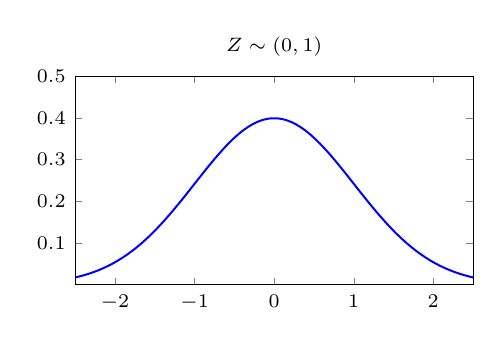
\begin{tikzpicture}[scale = 0.6]
       \begin{axis}[title = {$Z \sim \Gaussian(0,1)$}, tick label style={font=\scriptsize, scale = 1/0.6}, title style={font=\scriptsize, scale = 1/0.6},
    xtick={-2,-1,...,2},
    ytick = {0.1,0.2,0.3,0.4, 0.5},
    ymin=0,ymax=0.5,xmin=-2.5, xmax = 2.5, width=10cm, height=6cm]
    \addplot[very thick,domain=-3:3,blue, samples=100] {0.3989*e^(-x^2/2)};
    \end{axis}
    \end{tikzpicture}
    \end{minipage}%
    \begin{minipage}{0.5\textwidth}
        \centering
  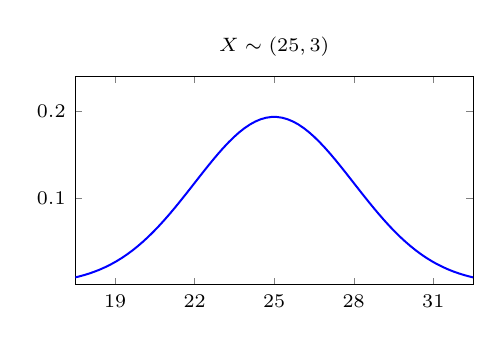
\begin{tikzpicture}[scale = 0.6]
       \begin{axis}[title = {$X \sim \Gaussian(25,3)$}, tick label style={font=\scriptsize, scale = 1/0.6}, title style={font=\scriptsize, scale = 1/0.6},
    ymin=0,ymax=0.24,xmin=17.5, xmax = 32.5, xtick = {19,22,25,28,31}, ytick = {0.1,0.2,0.3,0.4,0.5}, width=10cm, height=6cm]
       \addplot[very thick,domain=15:35,blue, samples =100] {0.19298*e^(-(x-25)^2/18)};
    \end{axis}
    \end{tikzpicture}
\end{minipage}
\end{center}
\end{definition}

The Gaussian distribution gets its name from mathematician Carl Friedrich Gauss, and is also known as the Normal distribution. It will play a central role in the estimation and testing procedures we'll develop in the next chapter. 

Unfortunately, the pdf $f_X$ for a Gaussian distribution is not integrable in elementary terms. In other words, its antiderivative can't be expressed using only the functions and operations you've encountered in Calculus II, which means we can't find areas under the curve (probabilities) using those methods.

The traditional way to get around this issue is to use a large table of values of the cdf as a reference. Unless otherwise stated, the letter $Z$ will be reserved for the random variable $Z \sim \Gaussian(0,1)$ from now on, and a $Z$-table is simply a large table of values of the cdf $F_Z(z) = P(Z \leq z)$ for many different realizations $z \in \mathbb{R}$.

What if $X$ is a Gaussian random variable with a nonzero mean and a standard deviation which is different from one? As you might expect given the two graphs shown above, it turns out the distributions of any two Gaussian random variables differ only by shifting and stretching. The tools required to show this are covered in the Probability \& Random Variables option course, 201-PRV.

\begin{proposition}If $X \sim \Gaussian (\mu,\sigma)$, then $Z = \frac{X - \mu}{\sigma} \sim \Gaussian(0,1)$.
\end{proposition}

The process of translating values of any Gaussian distributed random variable into corresponding values of $Z \sim \Gaussian (0,1)$ is known as \newterm{standardization}\index{Standardization}, and $Z \sim \Gaussian (0,1)$ is known as the \newterm{standard normal distribution}\index{Standard Normal Distribution}\index{Distribution!Standard Normal}. To standardize a realization $x$ of $X \sim \Gaussian(\mu, \sigma)$ we simply compute $z  = \frac{x - \mu}{\sigma}$, which is known as the \newterm{Z-score}\index{Z-score} of $x$, and we can treat the resulting $z$ as a realization of $Z \sim \Gaussian(0, 1)$.

\begin{example}\label{FemaleHeightsGaussian} The height of a randomly selected Canadian adult female, in inches, is approximated by the random variable $X \sim \Gaussian(64,2.5)$. What proportion of Canadian adult females are taller than 5'8"? What proportion have heights between 5'3" and 5'7"?

To standardize 5'8"\,=\,68", we calculate $z = \frac{68 - 64}{2.5} = 1.6$. Then we have
\
\begin{center}
    \begin{minipage}{0.5\textwidth}
        \centering
  $$\begin{aligned}P(X > 68) &= P(Z > 1.6) \\ &= 1 - P(Z \leq 1.6) \\ &= 1 - 0.9452 \\ &= 0.0548 \approx 5.5\%.\end{aligned}$$
  \vspace{1.25em}
    \end{minipage}\begin{minipage}{0.5\textwidth}
        \centering
   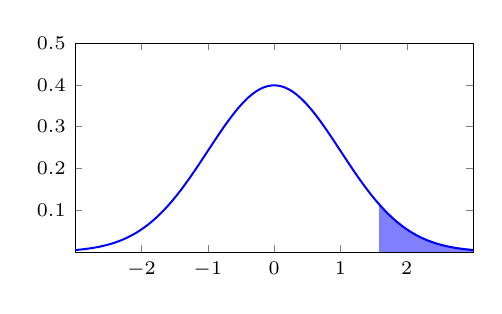
\begin{tikzpicture}[scale = 0.6]
       \begin{axis}[tick label style={font=\scriptsize, scale = 1/0.6}, ymin=0,ymax=0.5,xmin=-3, xmax = 3, xtick = {-2,-1,0,1,2}, ytick = {0.1,0.2,0.3,0.4,0.5}, width = 10cm, height = 6cm]
       \addplot[fill = blue, very thick,domain=1.6:3,blue!50, samples=100] {0.3989*e^(-x^2/2)}\closedcycle;
       \addplot[very thick,domain=-3:3,blue, samples=100] {0.3989*e^(-x^2/2)};
       \addplot[domain=-3:3] {0};
    \end{axis}
    \end{tikzpicture}
\end{minipage}
\end{center}

Thus, about 5.5\% of Canadian adult females are taller than 5'8". For the second part we standardize 5'3"\,=\,63" and 5'7"\,=\,67" to obtain $z_1 = \frac{63-64}{2.5} = -0.4$ and $z_2 = \frac{67-64}{2.5} = 1.2$, then calculate

\begin{center}
    \begin{minipage}{0.5\textwidth}
        \centering
  $$\begin{aligned}\qquad P(63 < X < 67) &= P(-0.4 < Z < 1.2) \\ &= P(Z \leq 1.2) - P(Z \leq -0.4) \\ &= 0.8849 - 0.3446 \\ &= 0.5404 \approx 54\%.\end{aligned}$$
  \vspace{1.25em}
    \end{minipage}\begin{minipage}{0.5\textwidth}
        \centering
   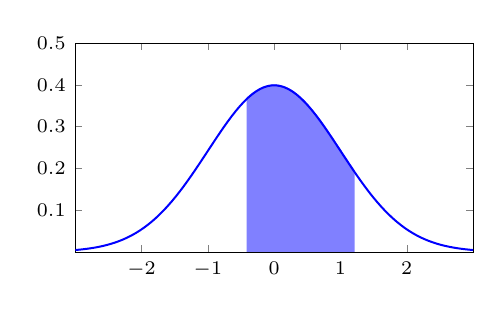
\begin{tikzpicture}[scale = 0.6]
       \begin{axis}[tick label style={font=\scriptsize, scale = 1/0.6}, ymin=0,ymax=0.5,xmin=-3, xmax = 3, xtick = {-2,-1,0,1,2}, ytick = {0.1,0.2,0.3,0.4,0.5}, width = 10cm, height = 6cm]
       \addplot[fill = blue, very thick,domain=-0.4:1.2,blue!50, samples=100] {0.3989*e^(-x^2/2)}\closedcycle;
       \addplot[very thick,domain=-3:3,blue, samples=100] {0.3989*e^(-x^2/2)};
       \addplot[domain=-3:3] {0};
    \end{axis}
    \end{tikzpicture}
\end{minipage}
\end{center}

Therefore, around 54\% of Canadian adult females are between 5'3" and 5'7".
\end{example}

Since there is now almost universal access to computers which can calculate areas under the pdf of $Z \sim \Gaussian(0,1)$ efficiently using numerical integration, $Z$-tables are something of a mathematical artifact whose uses are limited to classrooms and standardized tests.

\subsection*{Gaussian Distribution Shortcuts}

Any Gaussian distribution has two inflection points, and these occur precisely one standard deviation from the mean. This fact is useful when drawing a sketch of a Gaussian distribution.
\begin{center}    
    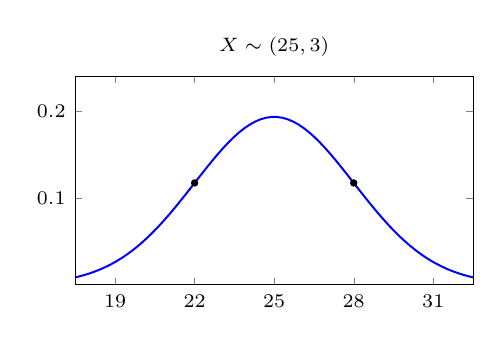
\begin{tikzpicture}[scale = 0.6]
       \begin{axis}[title = {$X \sim \Gaussian(25,3)$}, tick label style={font=\scriptsize, scale = 1/0.6}, title style={font=\scriptsize, scale = 1/0.6},
    ymin=0,ymax=0.24,xmin=17.5, xmax = 32.5, xtick = {19,22,25,28,31}, ytick = {0.1,0.2,0.3,0.4,0.5}, width=10cm, height=6cm]
       \addplot[very thick,domain=15:35,blue, samples =100] {0.19298*e^(-(x-25)^2/18)};
       \addplot [only marks] table {
28 0.11704
22 0.11704
};
    \end{axis}
    \end{tikzpicture}
 \end{center}

For approximate reasoning with Gaussian distributions without the aid of a $Z$-table or a computer, there is a well-known rule of thumb which is sometimes useful.

\begin{proposition}\index{68-95-99.7 Rule}\label{GaussianRuleThumb}(68-95-99.7 Rule) For any Gaussian distribution, 68\% of the area under its pdf occurs within one standard deviation of the mean, 95\% occurs within two standard deviations, and 99.7\% occurs within three standard deviations.
\begin{center}
  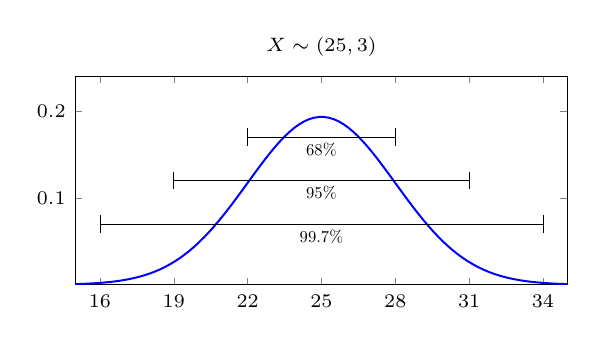
\begin{tikzpicture}[scale = 0.6]
       \begin{axis}[title = {$X \sim \Gaussian(25,3)$}, tick label style={font=\scriptsize, scale = 1/0.6}, title style={font=\scriptsize, scale = 1/0.6},
    ymin=0,ymax=0.24,xmin=15, xmax = 35, xtick = {16,19,22,25,28,31,34}, ytick = {0.1,0.2,0.3,0.4,0.5}, width=12cm, height=6cm]
       \addplot[very thick,domain=15:35,blue, samples =100] {0.19298*e^(-(x-25)^2/18)};
       \draw (axis cs:22,0.17) -- node[below]{68\%} (axis cs:28,0.17);
       \draw (axis cs:19,0.12) -- node[below]{95\%} (axis cs:31,0.12);
       \draw (axis cs:16,0.07) -- node[below]{99.7\%} (axis cs:34,0.07);
       \draw (axis cs:22,0.18) -- (axis cs:22,0.16);
       \draw (axis cs:28,0.18) -- (axis cs:28,0.16);
       \draw (axis cs:19,0.13) -- (axis cs:19,0.11);
       \draw (axis cs:31,0.13) -- (axis cs:31,0.11);
       \draw (axis cs:16,0.06) -- (axis cs:16,0.08);
       \draw (axis cs:34,0.06) -- (axis cs:34,0.08);
    \end{axis}
    \end{tikzpicture}
 \end{center}
\end{proposition}

Primarily used for quick approximate calculations, the rule also illustrates how quickly a Gaussian distribution approaches the horizontal axis when it moves away from its mean. To contrast this with the strange behaviour we saw in Example \ref{CauchyExpectation} at the end of the last section, we can say that Gaussian distributions have \newterm{thin tails}\index{Distribution! Thin-tailed}.

\begin{example}If $X \sim \Gaussian(64,2.5)$ is used to model the height of a randomly selected Canadian female, provide a range of heights which will include 95\% of all Canadian adult females.

Using the 68-95-99.7 Rule, $95\%$ of Canadian adult females will have heights within two standard deviations of the mean height, 64". So we calculate $64 - 2(2.5) = 59$ and $64 + 2(2.5) =69$, then conclude that 95\% of all Canadian adult females are taller than 59"\,=\,4'11" and shorter than 69"\,=\,5'9".
\end{example}

\section{Sampling Distributions}

Recall that a statistic is a numerical property of a sample, so the value of any statistic is determined by the sample it was derived from. Therefore, a statistic is a function whose input is a sample, and whose output is a real number.

If we fix a sample size, $n$, define a sample space $\Omega$ as the set of possible samples of that size, and assign probabilities to each possible sample, a statistic is a random variable defined on $\Omega$. This is the premise of \newterm{frequentist statistics}: a parameter is a real number, which we may or may not know, but a \emph{statistic is a random variable} and like any random variable, \emph{it has a distribution}.

\begin{definition}\index{Sampling Distribution}
The \newterm{sampling distribution} of a statistic, over samples of size $n$, is the distribution of possible values of that statistic.
\end{definition}

\begin{example}\label{DistOfMeanAge} Consider a population of three individuals, Alice, Bob, and Charles. Alice is 12 years old, Bob is 16 years old, and Charles is 22 years old. Let $\overline{X}$ denote the mean age in a sample of two individuals drawn from this population (now we're treating the sample mean as a random variable, so we write it as $\overline{X}$). Find the sampling distribution of $\overline{X}$ over all samples of size two taken with replacement.

\noindent If we let $X_1$ and $X_2$ denote the ages of the first and second individuals selected in our sample, then $\overline{X} = \frac{1}{2}(X_1 + X_2)$. There are $3\cdot3 = 9$ possible samples, which we enumerate below and for each, calculate the value of $\overline{X}$.

\begin{center}
\begin{tabular}{c|c|c|c}
Sample & $X_1$ & $X_2$ & $\overline{X}$ \\
\hline
A,A & $12$ & $12$ & $12$ \\
A,B & $12$ & $16$ & $14$ \\
A,C & $12$ & $22$ & $17$ \\
B,A & $16$ & $12$ & $14$ \\
B,B & $16$ & $16$ & $16$ \\
B,C & $16$ & $22$ & $19$ \\
C,A & $22$ & $12$ & $17$ \\
C,B & $22$ & $16$ & $19$ \\
C,C & $22$ & $22$ & $22$ \\
\end{tabular}
\end{center}

\noindent If we assume every sample is equally likely, then each of the nine samples above occurs with probability $\frac{1}{9}$, and we obtain the sampling distribution below.

\vspace{-1em}
\begin{center}
    \begin{minipage}{.45\textwidth}
        \centering
      \renewcommand*{\arraystretch}{1.35}
\begin{tabular}{c|c}
$x$ & $P(\overline{X} = x)$ \\
\hline
$12$ & $\frac{1}{9}$ \\
$14$ & $\frac{2}{9}$ \\
$16$ & $\frac{1}{9}$ \\
$17$ & $\frac{2}{9}$ \\
$19$ & $\frac{2}{9}$ \\
$22$ & $\frac{1}{9}$
\end{tabular}
\renewcommand*{\arraystretch}{1}
\vspace{0.25em}
    \end{minipage}%
    \begin{minipage}{0.5\textwidth}
        \centering
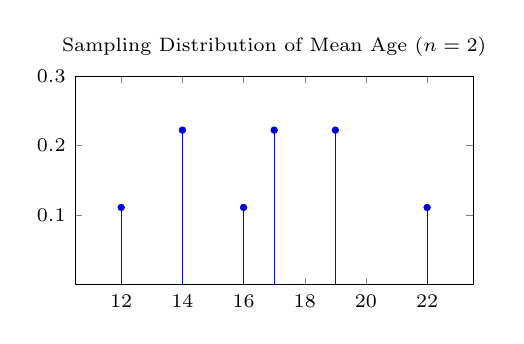
\begin{tikzpicture}[scale = 0.6]
\begin{axis} [title = {Sampling Distribution of Mean Age ($n=2$)}, width = 10cm, height = 6cm, ymin = 0, ymax = 0.3, xmin = 10.5, xmax = 23.5, tick label style={font=\scriptsize, scale = 1/0.6}, title style={font=\scriptsize, scale = 1/0.6}, ytick = {0.1,0.2,0.3}, xtick = {12,14,16,18,20,22}]
\addplot+[ycomb] plot coordinates {(12,0.1111) (14,0.2222) (16,0.1111) (17,0.2222) (19,0.2222) (22,0.1111)}; 
\end{axis}
\end{tikzpicture}
\end{minipage}
\end{center}
\begin{keypoint}
To create this distribution, we assigned equal probability to every possible sample, which means we are assuming random sampling (to be completely explicit, we're assuming the sampling process results in a simple random sample taken with replacement).
\end{keypoint}
If we compute the mean of this distribution, $E(\overline{X}) = 12 \cdot \frac{1}{9} + 14 \cdot \frac{2}{9} + \dots + 22 \cdot \frac{1}{9} = \frac{50}{3}$. Note that the mean age in our population is $\mu = \frac{12+16+22}{3} = \frac{50}{3}$ also. This is not a coincidence.
\end{example}

\begin{proposition}\label{MeanOfSampleMean}
If $\overline{X}$ is the mean of a random sample taken from a population with mean $\mu$, then $E(\overline{X}) = \mu$. In other words, the average sample mean, taken across all samples, is equal to the population mean.
\end{proposition}

\begin{remark}
The notation $\mu_{\overline{X}}$ is also used for $E(\overline{X})$, so you may see the result above written as $\mu_{\overline{X}} = \mu$.
\end{remark}

This is a key result that all the inference procedures in the next Chapter depend on, and it's a very special property of the mean that is generally not true of other statistics.

Now that we know that in any scenario where we're doing random sampling, the mean of the distribution of $\overline{X}$ is $\mu$, it's natural to wonder about the variance. Is there a simple relationship between the variance of $\overline{X}$ and the variance of the population the random sample was drawn from?

\begin{example}
Consider again the scenario in Example \ref{DistOfMeanAge}. Let's compute the variance of the random variable $\overline{X}$ and the compare it to the variance of the population.
$$\Var(\overline{X}) = (12 - \textstyle\frac{50}{3})^2 \cdot \frac{1}{9} + (14 - \textstyle\frac{50}{3})^2 \cdot \frac{2}{9} + \dots + (22 - \textstyle\frac{50}{3})^2 \cdot \frac{1}{9} = \frac{76}{9}$$
$$\sigma^2 = \textstyle\frac{1}{3}\left((12-\frac{50}{3})^2 + (16-\frac{50}{3})^2 + (22-\frac{50}{3})^2 \right) = \frac{152}{9}$$
In fact, the variance of $\overline{X}$ is precisely half the population variance. This is, again, not a coincidence.
\end{example}

\begin{proposition}\label{VarianceOfSampleMean}
If $\overline{X}$ is the mean of a random sample of $n$ individuals taken from a population with variance $\sigma^2$, then $\Var(\overline{X}) = \frac{\sigma^2}{n}$. In other words, the variance of the distribution of the sample mean is $n$ times smaller than the variance of the population.
\end{proposition}

\begin{remark}
The notation $\sigma_{\overline{X}}$ is used for the standard deviation of $\overline{X}$, so taking the square root of each side of $\Var(\overline{X}) = \frac{\sigma^2}{n}$, we obtain $\sigma_{\overline{X}} = \frac{\sigma}{\sqrt{n}}$.
\end{remark}

The proofs of Propositions \ref{MeanOfSampleMean} and \ref{VarianceOfSampleMean} require results on properties of expected value and variance that are developed in the Probability \& Random Variables option course, 201-PRV.

To sum up, we've learned some important things about the \emx{distribution of means of random samples}. In any scenario where we compute the mean of a random sample, the average sample mean is precisely equal to the population mean, and the variance of the distribution of sample means is $n$ times smaller than the variance of the population. 

%This implies that if we use the mean of random sample $\overline{X}$ to guess the value of the population mean $\mu$, the target value we're trying to hit is precisely in the center of the distribution of our guess, and the larger the sample size, the smaller the dispersion in the distribution of our guess, that is, the more the distribution of our guess clusters around its center. Bigger samples usually result in better guesses, as you would expect.

%Put Grphics here


\section{The Central Limit Theorem}

Now that we know the mean and variance of the sampling distribution of $\xbar$, what can we say about the shape? Consider, for example, the continuous random variable with density function $f_X(x) = \frac{1}{2}e^{-\frac{1}{2}x}$ on $[0,\infty)$. We can approximate the sampling distribution of $\xbar$ by taking ten thousand random samples, calculating their means, and plotting the results.

If we take samples of size one from the distribution of $X$, the distribution of sample means should look just like the distribution of $X$, since the mean of a single observation is that observation itself. We're just building a histogram for the distribution of $X$ by taking many realizations.
\begin{center}
    \begin{minipage}{.5\textwidth}
        \centering
  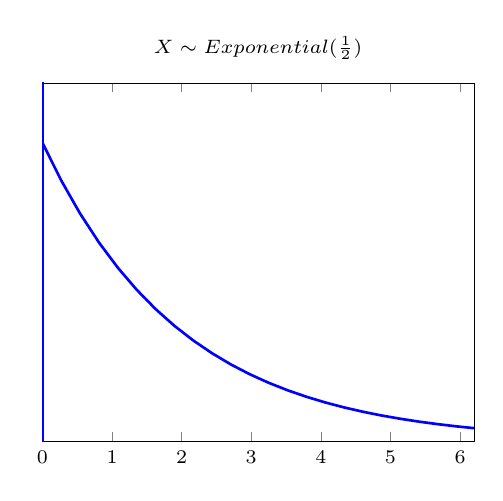
\begin{tikzpicture}[scale = 0.8]
       \begin{axis}[title = {$X \sim Exponential(\frac{1}{2})$},tick label style={font=\scriptsize, scale = 1/0.8}, title style={font=\scriptsize, scale = 1/0.8}, ymin=0,ymax=0.6,xmin=-0.0025, xmax = 6.2, xtick = {0,1,2,3,4,5,6}, ytick = {1}]
       \addplot[very thick,domain=0:6.5,blue] {0.5*e^(-0.5*x)};
       \draw[very thick, blue, -] (axis cs:0,0) -- (axis cs:0,2);
    \end{axis}
    \end{tikzpicture}
    \end{minipage}%
    \begin{minipage}{0.5\textwidth}
        \centering
  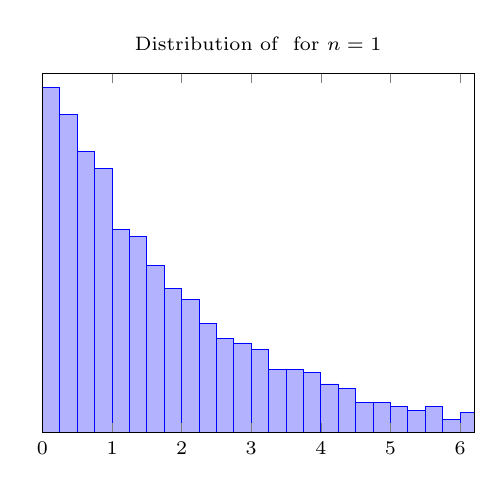
\begin{tikzpicture}[scale = 0.8]
\begin{axis}[title = {Distribution of $\xbar$ for $n=1$}, tick label style={font=\scriptsize, scale = 1/0.8}, title style={font=\scriptsize, scale = 1/0.8},ymin=0,ymax=1200,xmin=-0.0025, xmax = 6.2, xtick = {0,1,2,3,4,5,6}, ytick = {1500}, area style]
\addplot+[ybar interval,mark=no] plot coordinates {(0,1153) (0.25,1063) (0.5,939) (0.75,882) (1,678) (1.25,655) (1.5,557) (1.75,479) (2,443) (2.25,364) (2.5,313) (2.75,298) (3,275) (3.25,208) (3.5,211) (3.75,198) (4,161) (4.25,146) (4.5,99) (4.75,99) (5,86) (5.25,73) (5.5,86) (5.75,41) (6,65) (6.25,54)};
\end{axis}
\end{tikzpicture}
\end{minipage}
\end{center}
\begin{remark}
The continuous random variable $X$ with density function $f_X(x) = \frac{1}{2}e^{-\frac{1}{2}x}$ on $[0,\infty)$ is known as an exponential random variable with parameter $\frac{1}{2}$, which we can abbreviate $X \sim Exponential(\frac{1}{2})$. Exponential distributions are studied in detail in the Probability \& Random Variables option course, 201-PRV. For our purposes, it's simply a convenient distribution to use to illustrate the main result in this section. Note that $E(X) = \int_{0}^{\infty}\frac{1}{2}xe^{-\frac{1}{2}x}\,dx = 2$.
\end{remark}

What happens when we increase the sample size? Now we'll take ten thousand random samples, each consisting of two independent observations $X_1$ and $X_2$, and compute the mean $\xbar = \frac{1}{2}(X_1 + X_2)$ of each sample. The resulting distribution of sample means is given below on the right. Note that the most likely realizations of $X$ are very close to zero, but the most likely realizations of $\xbar$ are close to one. Each of the sample values $X_1$ and $X_2$ is more likely to be very close to zero than anywhere else, but samples where both values are simultaneously very close to zero are nonetheless quite unusual.
\begin{center}
    \begin{minipage}{.5\textwidth}
        \centering
  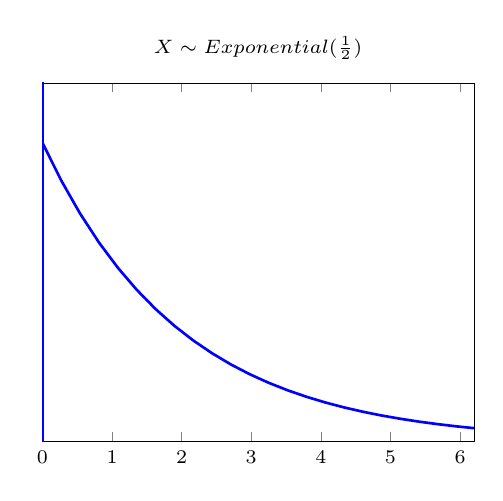
\begin{tikzpicture}[scale = 0.8]
       \begin{axis}[title = {$X \sim Exponential(\frac{1}{2})$}, tick label style={font=\scriptsize, scale = 1/0.8}, title style={font=\scriptsize, scale = 1/0.8},ymin=0,ymax=0.6,xmin=-0.0025, xmax = 6.2, xtick = {0,1,2,3,4,5,6}, ytick = {1}]
       \addplot[very thick,domain=0:6.5,blue] {0.5*e^(-0.5*x)};
       \draw[very thick, blue, -] (axis cs:0,0) -- (axis cs:0,2);
    \end{axis}
    \end{tikzpicture}
    \end{minipage}%
    \begin{minipage}{0.5\textwidth}
        \centering
  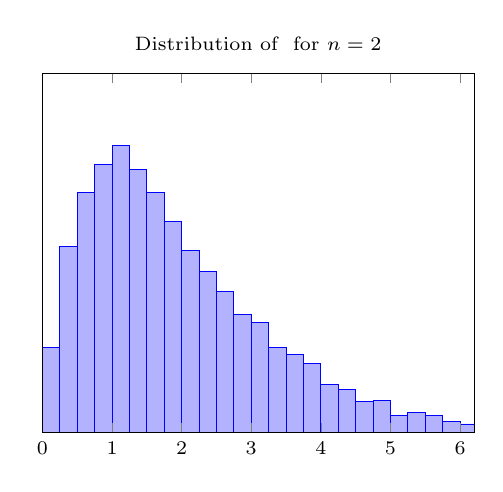
\begin{tikzpicture}[scale = 0.8]
\begin{axis}[title = {Distribution of $\xbar$ for $n=2$}, tick label style={font=\scriptsize, scale = 1/0.8}, title style={font=\scriptsize, scale = 1/0.8},ymin=0,ymax=1200,xmin=-0.0025, xmax = 6.2, xtick = {0,1,2,3,4,5,6}, ytick = {1500}, area style]
\addplot+[ybar interval,mark=no] plot coordinates {(0,282) (0.25,620) (0.5,801) (0.75,894) (1,959) (1.25,880) (1.5,803) (1.75,706) (2,608) (2.25,537) (2.5,469) (2.75,394) (3,366) (3.25,283) (3.5,260) (3.75,231) (4,158) (4.25,142) (4.5,103) (4.75,105) (5,57) (5.25,67) (5.5,57) (5.75,37) (6,27) (6.25,36)};
\end{axis}
\end{tikzpicture}
\end{minipage}
\end{center}
If we continue increasing the sample size, taking ten thousand random samples of larger and larger sizes from the same distribution, how will the distribution of the sample mean $\xbar$ change?
\begin{center}
    \begin{minipage}{.5\textwidth}
        \centering
  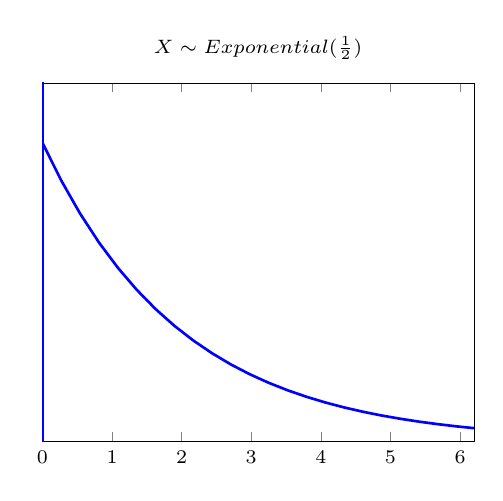
\begin{tikzpicture}[scale = 0.8]
       \begin{axis}[title = {$X \sim Exponential(\frac{1}{2})$},tick label style={font=\scriptsize, scale = 1/0.8}, title style={font=\scriptsize, scale = 1/0.8}, ymin=0,ymax=0.6,xmin=-0.0025, xmax = 6.2, xtick = {0,1,2,3,4,5,6}, ytick = {1}]
       \addplot[very thick,domain=0:6.5,blue] {0.5*e^(-0.5*x)};
       \draw[very thick, blue, -] (axis cs:0,0) -- (axis cs:0,2);
    \end{axis}
    \end{tikzpicture}
    \end{minipage}%
    \begin{minipage}{0.5\textwidth}
        \centering
  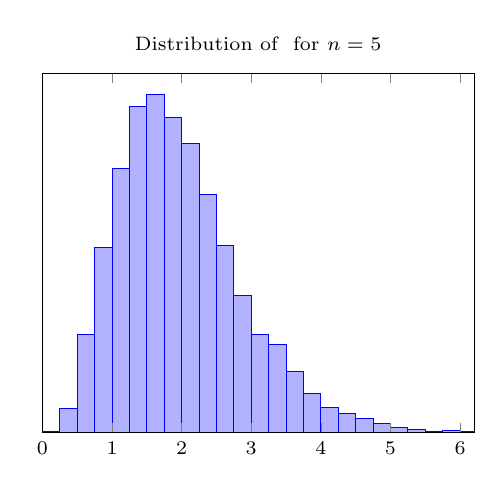
\begin{tikzpicture}[scale = 0.8]
\begin{axis}[title = {Distribution of $\xbar$ for $n=5$},tick label style={font=\scriptsize, scale = 1/0.8}, title style={font=\scriptsize, scale = 1/0.8}, ymin=0,ymax=1300,xmin=-0.0025, xmax = 6.2, xtick = {0,1,2,3,4,5,6}, ytick = {1500}, area style]
\addplot+[ybar interval,mark=no] plot coordinates {(0,4) (0.25,85) (0.5,355) (0.75,668) (1,954) (1.25,1180) (1.5,1224) (1.75,1140) (2,1045) (2.25,861) (2.5,678) (2.75,495) (3,354) (3.25,318) (3.5,218) (3.75,139) (4,89) (4.25,67) (4.5,49) (4.75,32) (5,17) (5.25,11) (5.5,4) (5.75,6) (6,2) (6.25,2)};
\end{axis}
\end{tikzpicture}
\end{minipage}
\end{center}
\begin{center}
    \begin{minipage}{.5\textwidth}
        \centering
  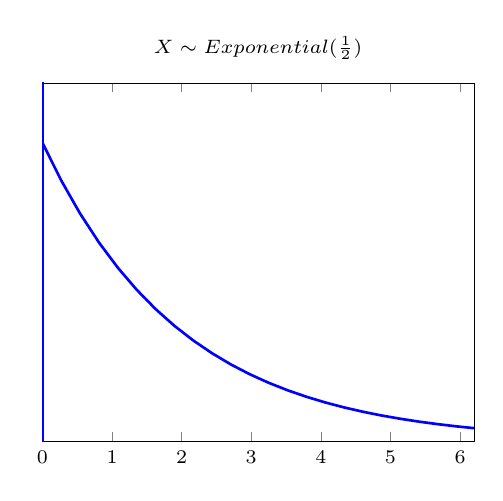
\begin{tikzpicture}[scale = 0.8]
       \begin{axis}[title = {$X \sim Exponential(\frac{1}{2})$},tick label style={font=\scriptsize, scale = 1/0.8}, title style={font=\scriptsize, scale = 1/0.8}, ymin=0,ymax=0.6,xmin=-0.0025, xmax = 6.2, xtick = {0,1,2,3,4,5,6}, ytick = {1}]
       \addplot[very thick,domain=0:6.5,blue] {0.5*e^(-0.5*x)};
       \draw[very thick, blue, -] (axis cs:0,0) -- (axis cs:0,2);
    \end{axis}
    \end{tikzpicture}
    \end{minipage}%
    \begin{minipage}{0.5\textwidth}
        \centering
  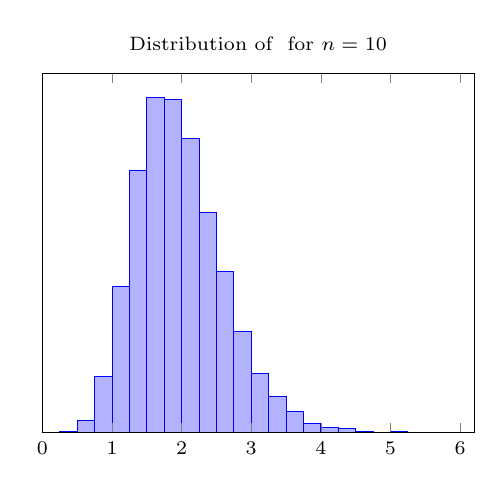
\begin{tikzpicture}[scale = 0.8]
\begin{axis}[title = {Distribution of $\xbar$ for $n=10$},tick label style={font=\scriptsize, scale = 1/0.8}, title style={font=\scriptsize, scale = 1/0.8}, ymin=0,ymax=1750,xmin=-0.0025, xmax = 6.2, xtick = {0,1,2,3,4,5,6}, ytick = {2000}, area style]
\addplot+[ybar interval,mark=no] plot coordinates {(0,0) (0.25,1) (0.5,55) (0.75,269) (1,709) (1.25,1275) (1.5,1631) (1.75,1624) (2,1434) (2.25,1073) (2.5,782) (2.75,493) (3,288) (3.25,175) (3.5,102) (3.75,42) (4,22) (4.25,18) (4.5,5) (4.75,0) (5,2) (5.25,0) (5.5,0) (5.75,0) (6,0) (6.25,0)};
\end{axis}
\end{tikzpicture}
\end{minipage}
\end{center}
\begin{center}
    \begin{minipage}{.5\textwidth}
        \centering
  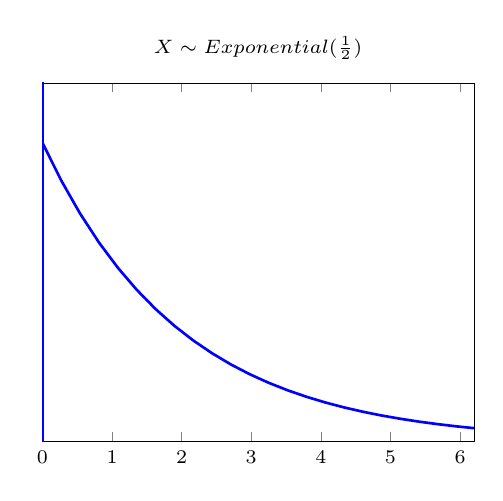
\begin{tikzpicture}[scale = 0.8]
       \begin{axis}[title = {$X \sim Exponential(\frac{1}{2})$},tick label style={font=\scriptsize, scale = 1/0.8}, title style={font=\scriptsize, scale = 1/0.8}, ymin=0,ymax=0.6,xmin=-0.0025, xmax = 6.2, xtick = {0,1,2,3,4,5,6}, ytick = {1}]
       \addplot[very thick,domain=0:6.5,blue] {0.5*e^(-0.5*x)};
       \draw[very thick, blue, -] (axis cs:0,0) -- (axis cs:0,2);
    \end{axis}
    \end{tikzpicture}
    \end{minipage}%
    \begin{minipage}{0.5\textwidth}
        \centering
  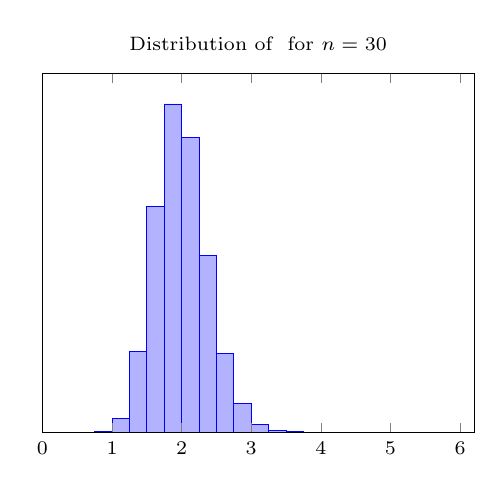
\begin{tikzpicture}[scale = 0.8]
\begin{axis}[title = {Distribution of $\xbar$ for $n=30$},tick label style={font=\scriptsize, scale = 1/0.8}, title style={font=\scriptsize, scale = 1/0.8}, ymin=0,ymax=2900,xmin=-0.0025, xmax = 6.2, xtick = {0,1,2,3,4,5,6}, ytick = {3000}, area style]
\addplot+[ybar interval,mark=no] plot coordinates {(0,0) (0.25,0) (0.5,0) (0.75,6) (1,108) (1.25,653) (1.5,1826) (1.75,2653) (2,2385) (2.25,1430) (2.5,636) (2.75,230) (3,59) (3.25,12) (3.5,2) (3.75,0) (4,0) (4.25,0) (4.5,0) (4.75,0) (5,0) (5.25,0) (5.5,0) (5.75,0) (6,0) (6.25,0)};
\end{axis}
\end{tikzpicture}
\end{minipage}
\end{center}

In the last section, we saw that if $\xbar$ is the mean of a random sample, then $E(\xbar) = \mu$ and $\Var(\xbar) = \frac{\sigma^2}{n}$. These results are visible in the graphics above. Each distribution of $\xbar$ is centered at 2, which is the mean of the exponential distribution the samples were drawn from, and the dispersion of the distribution of $\xbar$ decreases as the sample size grows (note that $\frac{\sigma^2}{n}$ is a decreasing function of $n$).

Moreover, there is a clear trend in the shapes of the sampling distributions. As the sample size increases, the distribution looks less like an exponential distribution, and more like a Gaussian distribution. This, once again, is not a coincidence.

This phenomenon is why the Gaussian distribution plays such a central role in statistics. If some quantity is obtained by averaging a random sample, and the sample size is large enough, then we know that the distribution of that quantity must be approximately Gaussian \emph{regardless of the shape of the distribution the sample values were drawn from}.

\begin{theorem} (\newterm{Central Limit Theorem})\index{Central Limit Theorem}\label{CLT} Consider a variable with mean $\mu$ and standard deviation $\sigma$ in some population, and let $\xbar$ denote the mean of a random sample of $n$ values drawn from that population. Then as the sample size $n$ increases, the sampling distribution of $\xbar$ becomes better approximated by $\Gaussian(\muxbar,\sigmaxbar)$, where $\mu_{\xbar} = \mu$ and $\sigma_{\xbar} = \frac{\sigma}{\sqrt{n}}$.
\end{theorem}

The conclusion of the theorem is written here in very informal language. To make it more precise, we would need to decide on a way to measure the difference between two distributions, so the theorem above could state that this difference vanishes as $n \to \infty$. For details, see \cite{DevoreBerk} or \cite{Ghahramani}.

We will write $Y \sim AG(\mu,\sigma)$ to indicate a random variable $Y$ has a distribution which is approximately Gaussian with mean $\mu$ and standard deviation $\sigma$. This way, the conclusion of the central limit theorem can be written simply as $\xbar \sim AG(\mu,\frac{\sigma}{\sqrt{n}})$, where $\mu$ and $\sigma$ are the mean and standard deviation of the population our sample was drawn from.

\begin{example}\label{CLTExamp}Twenty numbers in the interval $[0,1]$ are independently chosen uniformly at random. What is the probability their sum is higher than eight?

In order to use the central limit theorem, we need to formulate this question in terms of the mean of a sample. In this case, we have a sample of $n=20$ values drawn from a uniform distribution on the interval $[0,1]$. Observe that
$$X_1 + X_2 + \cdots + X_{20} > 8 \ \ \rightarrow \ \  \frac{X_1 + X_2 + \cdots + X_{20} }{20} > \frac{8}{20}.$$

Thus, to answer this question, we need to find the probability of obtaining a sample of twenty values with a mean $\xbar$ higher than $\frac{2}{5}$. We know from Example \ref{MeanVarianceUnitInterval} that the mean and standard deviation of the distribution our sample is drawn from are $\mu = \frac{1}{2}$ and $\sigma = \frac{1}{\sqrt{12}}$.

The central limit theorem states that the distribution of $\xbar$ is approximately Gaussian, with a mean of $\mu = \frac{1}{2}$ and a standard deviation of $\frac{\sigma}{\sqrt{n}} = \frac{1}{\sqrt{12}\sqrt{20}} = \frac{1}{\sqrt{240}}$, or more concisely, $\xbar \sim AG(\frac{1}{2}, \frac{1}{\sqrt{240}})$.

Now the probability of obtaining a sample with $\xbar$ higher than $\frac{2}{5}$ can be calculated (approximately) by standardizing and using a $Z$-table.
$$z = \frac{\xbar - \muxbar}{\sigmaxbar} = \frac{\frac{2}{5} - \frac{1}{2}}{\frac{1}{\sqrt{240}}} \approx -1.55$$
\begin{center}
    \begin{minipage}{.5\textwidth}
        \centering
  \eqns{P(\xbar > \textstyle\frac{2}{5}) &= P(Z > -1.55) \\ &= 1 - P(Z \leq -1.55) \\ &= 1 - 0.0603 \\ &= 0.9397 \approx 94\%}
  \vspace{1.25em}
    \end{minipage}%
    \begin{minipage}{0.5\textwidth}
        \centering
   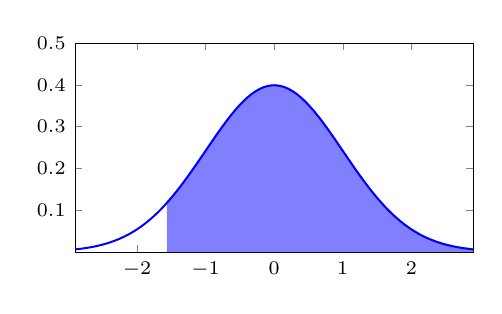
\begin{tikzpicture}[scale = 0.6]
       \begin{axis}[width = 10cm, height = 6cm, tick label style={font=\scriptsize, scale = 1/0.6}, ymin=0,ymax=0.5,xmin=-2.9, xmax = 2.9, xtick = {-2,-1,0,1,2}, ytick = {0.1,0.2,0.3,0.4,0.5}]
       \addplot[fill = blue, very thick,domain=-1.55:3,blue!50, samples=100] {0.3989*e^(-x^2/2)}\closedcycle;
       \addplot[very thick,domain=-3:3,blue, samples=100] {0.3989*e^(-x^2/2)};
       \addplot[domain=-3:3] {0};
    \end{axis}
    \end{tikzpicture}
\end{minipage}
\end{center}

Note that the central limit theorem does not tell us how accurate the Gaussian approximation of the distribution of $\xbar$ is, just that it will be more accurate for larger sample sizes. Let's take ten thousand samples of twenty numbers in the interval $[0,1]$ and plot the resulting sampling distribution of $\xbar$, along with the approximating normal distribution given by the central limit theorem.

If the two distributions match well, then we'll know that our answer above is fairly accurate. If the sampling distribution is still far from being Gaussian, then we'll have to disregard our answer.
\begin{center}
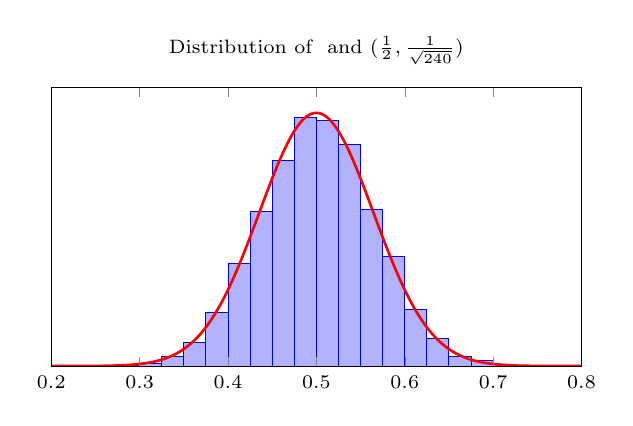
\begin{tikzpicture}[scale = 0.8]
\begin{axis}[title = {Distribution of $\xbar$ and $\Gaussian(\frac{1}{2},\frac{1}{\sqrt{240}})$}, tick label style={font=\scriptsize, scale = 1/0.8}, title style={font=\scriptsize, scale = 1/0.8}, ymin=0,ymax=1700,xmin=0.2, xmax = 0.8, xtick = {0.2,0.3,0.4,0.5,0.6,0.7,0.8}, ytick = {3300}, area style, width = 10cm, height = 6cm]
\addplot+[ybar interval,mark=no] plot coordinates {(0,0) (0.025,0) (0.05,0) (0.075,0) (0.1,0) (0.125,0) (0.15,0) (0.175,0) (0.2,0) (0.225,0) (0.25,2) (0.275,6) (0.3,13) (0.325,61) (0.35,147) (0.375,328) (0.4,624) (0.425,942) (0.45,1257) (0.475,1520) (0.5,1499) (0.525,1355) (0.55,955) (0.575,668) (0.6,346) (0.625,167) (0.65,58) (0.675,34) (0.7,7) (0.725,0)};
\addplot[very thick,domain=0:1,red, samples=500] {250*6.185*e^((-(x - 0.5)^2)/(2*(1/240)))};
\end{axis}
\end{tikzpicture}
\end{center}
The distribution of $\xbar$ for random samples of size twenty is extremely well approximated by a Gaussian distribution, so we can be sure our answer is reasonably accurate.
\end{example}

\subsection*{Sample Size}

The central limit theorem states that the sampling distribution of $\xbar$ will eventually look Gaussian, once the sample size is large enough. The question is then how large must our sample be, so that using a Gaussian distribution for probability calculations, as in the example above, gives an accurate result?

Unfortunately, the answer depends on the details of the population distribution. Symmetric population distributions with tails that decay exponentially (thin tails) typically yield sampling distributions for $\xbar$ which are very close to Gaussian even for single digit sample sizes, while asymmetric population distributions with tails that decay polynomially (fat tails) can result in sampling distributions for $\xbar$ which don't look Gaussian until the sample size becomes extremely large.

As a rule of thumb, we'll require a sample size of thirty or more to treat the distribution of $\xbar$ as if it's Gaussian. There is nothing mathematically significant about this value, or slightly different values you might find in other texts. We're simply establishing a clear, yet arbitrary, baseline. 

\begin{remark}
If the population distribution is known to be Gaussian, then any sample size will suffice. In fact, an important property of Gaussian distributions is that the average of any number of observations from a Gaussian distribution is again Gaussian, no central limit theorem required.
\end{remark}

In practice, to convince themselves the sampling distribution of $\xbar$ is sufficiently close to a Gaussian distribution for a given sample size $n$, statisticians could either rigorously derive error bounds from some known properties of the population distribution, usually in combination with stronger variations of the central limit theorem, or use statistical software to take many samples from an educated guess at the population distribution, and approximate the sampling distribution empirically, as was done to generate the graphics at the beginning of this section.

\begin{example}
If a biased coin with a 55\% probability of heads is flipped one hundred times, what is the probability that the number of heads observed is less than the number of tails?

If we call a head a success, then we have a sample of $n=100$ values $X_1,X_2\,\dots\,,X_{100}$ from $X \sim \Bernoulli(0.55)$. If more tails than heads were observed, this means that more than half of the $X_i$ are zeros, so $\xbar = \frac{X_1 + X_2 + \cdots + X_{100}}{100} < \frac{50}{100} =0.5$.

Using the formulas for the mean and variance of a Bernoulli random variable in Proposition \ref{BernoulliExpectation}, the mean and standard deviation of the sampling distribution of $\xbar$ are given by 
$$\muxbar = \mu = p = 0.55 \ \ \text{and} \ \  \sigmaxbar = \frac{\sigma}{\sqrt{n}} = \frac{\sqrt{p(1-p)}}{\sqrt{n}} = \textstyle\frac{\sqrt{0.55\cdot 0.45}}{\sqrt{100}} \approx 0.05.$$

By the central limit theorem, $\xbar \sim AG(0.55,0.05)$, so we can calculate (approximately) the probability of obtaining a sample whose mean is smaller than $0.5$ by standardizing and using a $Z$-table.
$$z = \frac{\xbar - \muxbar}{\sigmaxbar} = \frac{0.5 - 0.55}{0.05} = \frac{-0.05}{0.05} = -1$$

\begin{center}
    \begin{minipage}{.5\textwidth}
        \centering
  \eqns{P(\xbar < 0.5) &= P(Z < -1) \\ &= 0.1587 \approx 16\%}
  \vspace{1.25em}
    \end{minipage}%
    \begin{minipage}{0.5\textwidth}
        \centering
   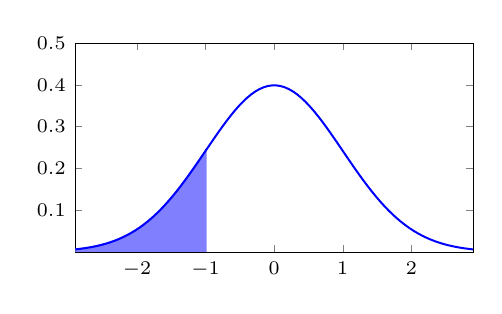
\begin{tikzpicture}[scale = 0.6]
       \begin{axis}[width = 10cm, height = 6cm, tick label style={font=\scriptsize, scale = 1/0.6}, ymin=0,ymax=0.5,xmin=-2.9, xmax = 2.9, xtick = {-2,-1,0,1,2}, ytick = {0.1,0.2,0.3,0.4,0.5}]
       \addplot[fill = blue, very thick,domain=-3:-1,blue!50, samples=100] {0.3989*e^(-x^2/2)}\closedcycle;
       \addplot[very thick,domain=-3:3,blue, samples=100] {0.3989*e^(-x^2/2)};
       \addplot[domain=-3:3] {0};
    \end{axis}
    \end{tikzpicture}
\end{minipage}
\end{center}
Therefore, there's about a $16\%$ chance we will observe more tails than heads. \\
\end{example}

\begin{warning}
It's very important to know the hypotheses of the central limit theorem. The procedures introduced in the next chapter are justified so long as we can treat the mean of our sample as a realization of a Gaussian random variable, which we can as long as these statements hold.
\begin{itemize}
\item The sample data we're working with was obtained via random sampling.
\item The sample data came from a distribution with well-defined mean and variance.
\item The sample size is large enough, or our sample data came from a Gaussian distribution.
\end{itemize}
\end{warning}


%Error of Average of guesses vs Average of Guess errors illustrates CLT




